%*****************************************
\chapter{Fundamental Skills}\label{ch01:fundamental_skills}
%*****************************************

Microsoft® Excel® is a tool that can be used in virtually all careers and is valuable in both professional and personal settings. Whether you need to keep track of medications in inventory for a hospital or create a financial plan for your retirement, Excel enables you to do these activities efficiently and accurately. This chapter introduces the fundamental skills necessary to get you started in using Excel. You will find that just a few skills can make you very productive in a short period of time.

\section{Overview of Microsoft Excel}

\begin{center}
	\begin{objbox}{Learning Objectives}
		\begin{itemize}
			\setlength{\itemsep}{0pt}
			\setlength{\parskip}{0pt}
			\setlength{\parsep}{0pt}
			
			\item Examine the value of using Excel to make decisions.
			\item Learn how to start Excel.
			\item Become familiar with the Excel workbook.
			\item Understand how to navigate worksheets.
			\item Examine the Excel Ribbon.
			\item Examine the right-click menu options.
			\item Learn how to save workbooks.
			\item Examine the Status Bar.
			\item Become familiar with the features in the Excel Help window.
			
		\end{itemize}
	\end{objbox}
\end{center}

Microsoft® Office contains a variety of tools that help people accomplish many personal and professional objectives. Microsoft Excel is perhaps the most versatile and widely used of all the Office applications. No matter which career path you choose, you will likely need to use Excel to accomplish your professional objectives, some of which may occur daily. This chapter provides an overview of the Excel application along with an orientation for accessing the commands and features of an Excel workbook.

\subsection{Making Decisions With Excel}

Taking a very simple view, Excel is a tool that allows you to enter quantitative data into an electronic spreadsheet to apply one or many mathematical computations. These computations ultimately convert that quantitative data into information. The information produced in Excel can be used to make decisions in both professional and personal contexts. For example, employees can use Excel to determine how much inventory to buy for a clothing retailer, how much medication to administer to a patient, or how much money to spend to stay within a budget. With respect to personal decisions, you can use Excel to determine how much money you can spend on a house, how much you can spend on car lease payments, or how much you need to save to reach your retirement goals. We will demonstrate how you can use Excel to make these decisions and many more throughout this text.

Figure \ref{01:fig01} shows a completed Excel worksheet that will be constructed in this chapter. The information shown in this worksheet is top-line sales data for a hypothetical merchandise retail company. The worksheet data can help this retailer determine the number of salespeople needed for each month, how much inventory is needed to satisfy sales, and what types of products should be purchased.

\begin{figure}[H]
	\centering
	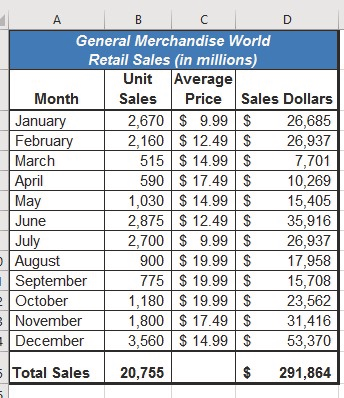
\includegraphics[width=\maxwidth{.95\linewidth}]{gfx/ch01_fig01}
	\caption{Example of an Excel Worksheet}
	\label{01:fig01}
\end{figure}

\subsection{Starting Excel}

\begin{enumerate}
	\item Locate Excel on your computer.
	\item Click Microsoft Excel to launch the Excel application and present you with workbook options.
	\item Click the first option; “Blank Workbook”.
\end{enumerate}

\subsection{The Excel Workbook}

Once Excel is started, a blank workbook will open on your screen. A workbook is an Excel file that contains one or more worksheets (sometimes referred to as spreadsheets). Excel will assign a file name to the workbook, such as \textbf{Book1}, \textbf{Book2}, \textbf{Book3}, and so on, depending on how many new workbooks are opened. Figure \ref{01:fig02} shows a blank workbook after starting Excel. Take some time to familiarize yourself with this screen. Your screen may be slightly different based on the version being used.

\begin{figure}[H]
	\centering
	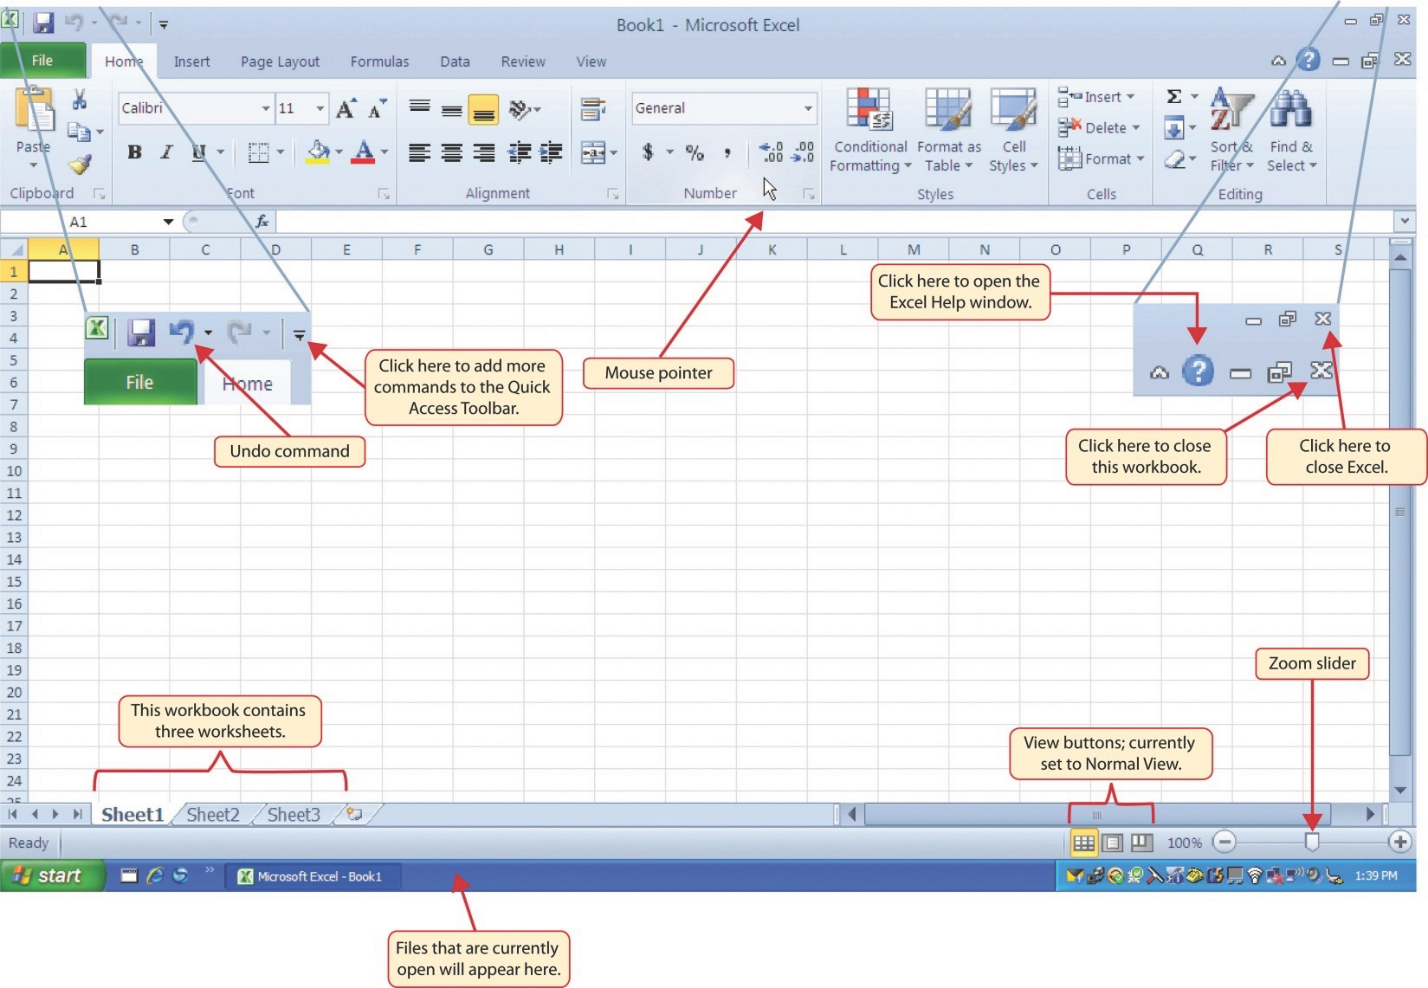
\includegraphics[width=\maxwidth{.95\linewidth}]{gfx/ch01_fig02}
	\caption{Blank Workbook}
	\label{01:fig02}
\end{figure}

Your workbook should already be maximized (or shown at full size) once Excel is started, as shown in Figure \ref{01:fig02}. However, if your screen looks like Figure \ref{01:fig03} after starting Excel, you should click the Maximize button, as shown in the figure.

\begin{figure}[H]
	\centering
	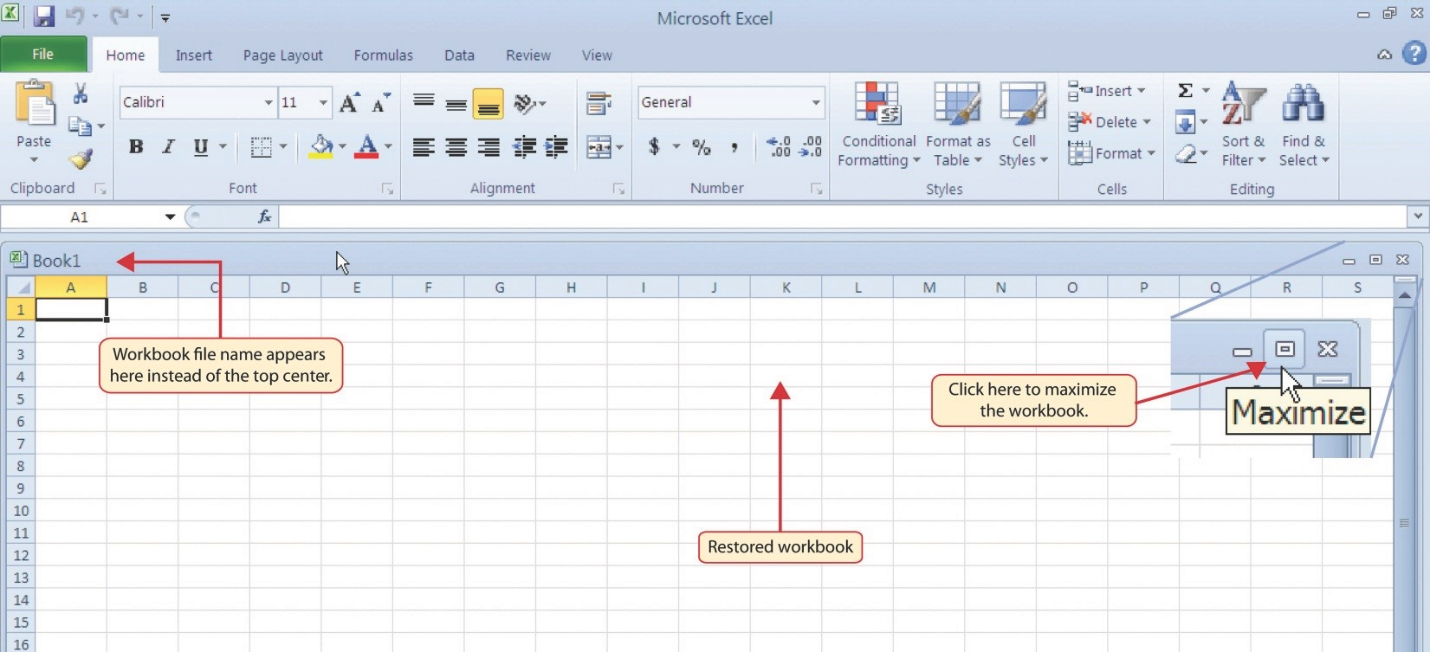
\includegraphics[width=\maxwidth{.95\linewidth}]{gfx/ch01_fig03}
	\caption{Restored Worksheet}
	\label{01:fig03}
\end{figure}

\subsection{Navigating Worksheets}

Data are entered and managed in an Excel worksheet. The worksheet contains several rectangles called cells for entering numeric and nonnumeric data. Each cell in an Excel worksheet contains an address, which is defined by a column letter followed by a row number. For example, the cell that is currently activated in Figure \ref{01:fig03} is \textsf{A1}. This would be referred to as cell location \textsf{A1} or cell reference \textsf{A1}. The following steps explain how you can navigate in an Excel worksheet:

\begin{itemize}
	\item Place your mouse pointer over cell \textsf{D5} and left click.
	\item Check to make sure column letter D and row number 5 are highlighted, as shown in Figure \ref{01:fig04}.
\end{itemize}

\begin{figure}[H]
	\centering
	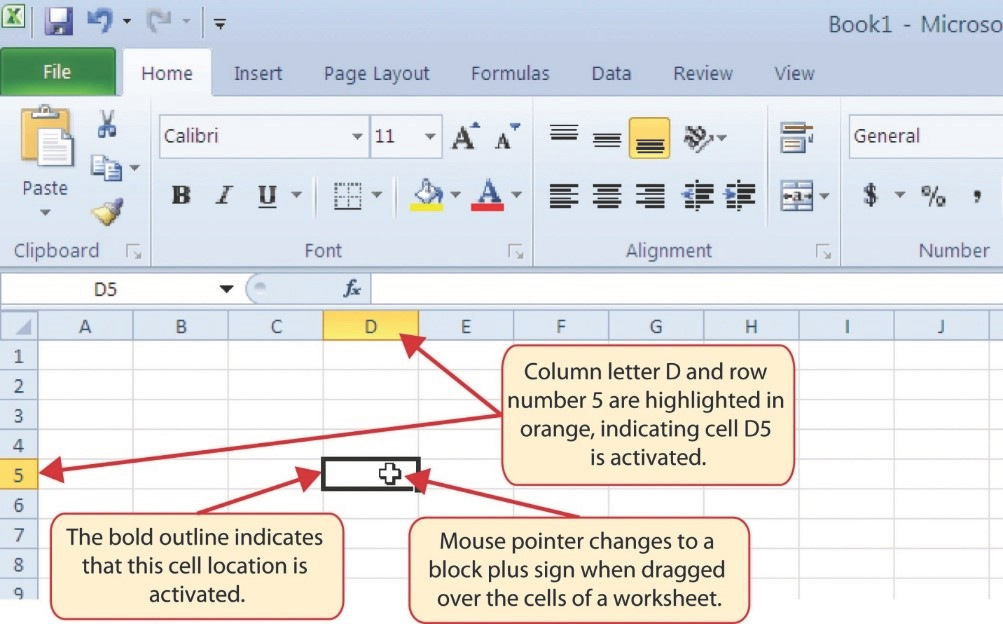
\includegraphics[width=\maxwidth{.95\linewidth}]{gfx/ch01_fig04}
	\caption{Activating a Cell Location}
	\label{01:fig04}
\end{figure}

\begin{enumerate}
	\item Move the mouse pointer to cell \textsf{A1}.
	\item Click and hold the left mouse button and drag the mouse pointer back to cell \textsf{D5}.
	\item Release the left mouse button. You should see several cells highlighted, as shown in Figure \ref{01:fig05}.
\end{enumerate}

This is referred to as a cell range and is documented as follows: \textsf{A1:D5}. Any two cell locations separated by a colon are known as a cell range. The first cell is the top left corner of the range, and the second cell is the lower right corner of the range.

\begin{figure}[H]
	\centering
	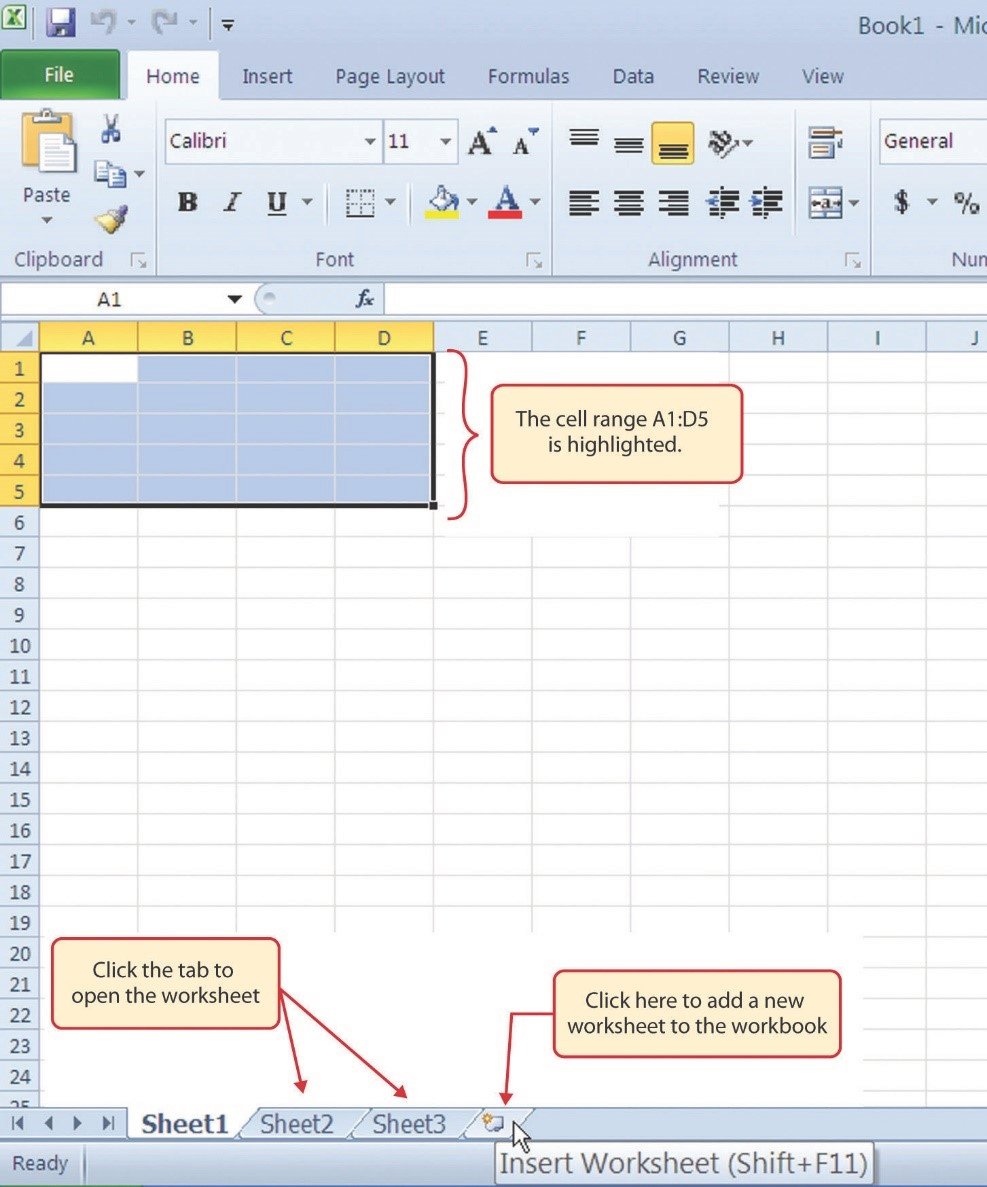
\includegraphics[width=\maxwidth{.95\linewidth}]{gfx/ch01_fig05}
	\caption{Highlighting a Range of Cells}
	\label{01:fig05}
\end{figure}

\begin{enumerate}
	\item At the bottom of the screen, you'll see worksheets. Depending on your version of Excel, you will see either three as displayed in Figure \ref{01:fig05} or just one. If you only have one sheet, click the ``Insert Worksheet'' to add a worksheet. Depending on your version, you instead may have a \textsf{+} sign; a click on the \textsf{+} adds an additional worksheet as well. This is how you open or add a worksheet within a workbook. Add another worksheet so that you now have three sheets displaying here.
	\item Click the \textit{Sheet1} worksheet tab at the bottom of the worksheet to return to the worksheet shown in Figure \ref{01:fig05}.
\end{enumerate}

\begin{center}
	\begin{shtcutbox}{Keyboard Shortcuts}
		\textbf{Basic Worksheet Navigation}
		\\
		\begin{itemize}
			\setlength{\itemsep}{0pt}
			\setlength{\parskip}{0pt}
			\setlength{\parsep}{0pt}

			\item Use the arrow keys on your keyboard to activate cells on the worksheet.
			\item Hold the \keystroke{Shift} key and press the arrow keys on your keyboard to highlight a range of cells in a worksheet.
			\item Hold the \keystroke{Ctrl} key while pressing the \keystroke{Page Down} or \keystroke{Page Up} keys to open other worksheets in a workbook.

		\end{itemize}
	\end{shtcutbox}
\end{center}

\subsection{The Excel Ribbon}

Excel's features and commands are found in the Ribbon, which is the upper area of the Excel screen that contains several tabs running across the top. Each tab provides access to a different set of Excel commands. Figure \ref{01:fig06} shows the commands available in the Home tab of the Ribbon. Table \ref{01:tab01}, ``Command Overview for Each Tab of the Ribbon,'' provides an overview of the commands that are found in each tab of the Ribbon.

\begin{figure}[H]
	\centering
	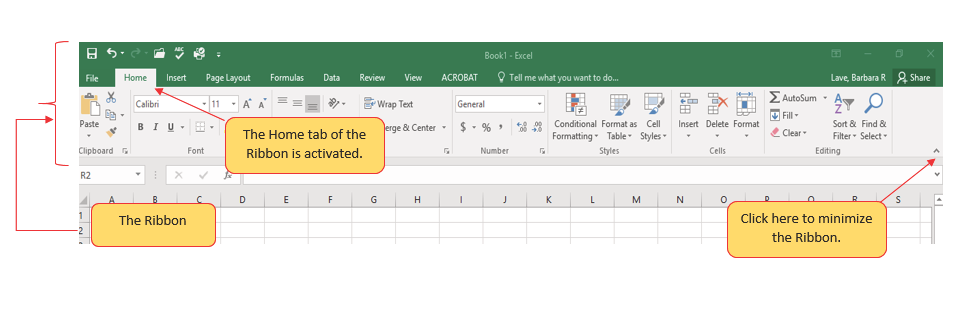
\includegraphics[width=\maxwidth{.95\linewidth}]{gfx/ch01_fig06}
	\caption{Home Tab of the Ribbon}
	\label{01:fig06}
\end{figure}

\begin{table}[H]
	\centering
	\definecolor{ltgray}{gray}{0.95} % this is a light gray
	\rowcolors{1}{}{ltgray} % zebra striping background
	\begin{tabularx}{0.95\linewidth}{
			p{0.15\linewidth}
			p{0.85\linewidth}}
		\toprule
		\textbf{Tab} & \textbf{Description} \\
		\midrule

		File & Also known as the Backstage view of the Excel workbook. Contains all commands for opening, closing, saving, and creating new Excel workbooks. Includes print commands, document properties, e-mailing options, and help features. The default settings and options are also found in this tab.\\

		Home & Contains the most frequently used Excel commands. Formatting commands are found in this tab along with commands for cutting, copying, pasting, and for inserting and deleting rows and columns.\\

		Insert & Used to insert objects such as charts, pictures, shapes, PivotTables, Internet links, symbols, or text boxes.\\
		
		Page Layout & Contains commands used to prepare a worksheet for printing. Also includes commands used to show and print the gridlines on a worksheet.\\
		
		Formulas & Includes commands for adding mathematical functions to a worksheet. Also contains tools for auditing mathematical formulas.\\

		Data & Used when working with external data sources such as Microsoft® Access®, text files, or the Internet. Also contains sorting commands and access to scenario tools.\\
		
		Review & Includes Spelling and Track Changes features. Also contains protection features to password protect worksheets or workbooks.\\
		
		View & Used to adjust the visual appearance of a workbook. Common commands include the Zoom and Page Layout view.\\
		
		\bottomrule
	\end{tabularx}
	\caption{Command Overview for Ribbon Tabs}
	\label{01:tab01}
\end{table}

The Ribbon shown in Figure \ref{01:fig06} is full, or maximized. The benefit of having a full Ribbon is that the commands are always visible while you are developing a worksheet. However, depending on the screen dimensions of your computer, you may find that the Ribbon takes up too much vertical space on your worksheet. If this is the case, you can minimize the Ribbon by clicking the button shown in Figure \ref{01:fig06}. When minimized, the Ribbon will show only the tabs and not the command buttons. When you click on a tab, the command buttons will appear until you select a command or click anywhere on your worksheet.

\begin{center}
	\begin{shtcutbox}{Keyboard Shortcuts}
		\textbf{Minimizing or Maximizing the Ribbon}
		\\
		\begin{itemize}
			\setlength{\itemsep}{0pt}
			\setlength{\parskip}{0pt}
			\setlength{\parsep}{0pt}
			
			\item Hold down the \keystroke{Ctrl} key and press the \keystroke{F1} key.
			\item Hold down the \keystroke{Ctrl} key and press the \keystroke{F1} key again to maximize the Ribbon.
			
		\end{itemize}
	\end{shtcutbox}
\end{center}

\subsection{Quick Access Toolbar and Right-Click Menu}

The Quick Access Toolbar is found at the upper left side of the Excel screen above the Ribbon, as shown in Figure \ref{01:fig07}. This area provides access to the most frequently used commands, such as Save and Undo. You also can customize the Quick Access Toolbar by adding commands that you use on a regular basis. By placing these commands in the Quick Access Toolbar, you do not have to navigate through the Ribbon to find them. To customize the Quick Access Toolbar, click the down arrow as shown in Figure \ref{01:fig07}. This will open a menu of commands that you can add to the Quick Access Toolbar. If you do not see the command you are looking for on the list, select the More Commands option.

\begin{figure}[H]
	\centering
	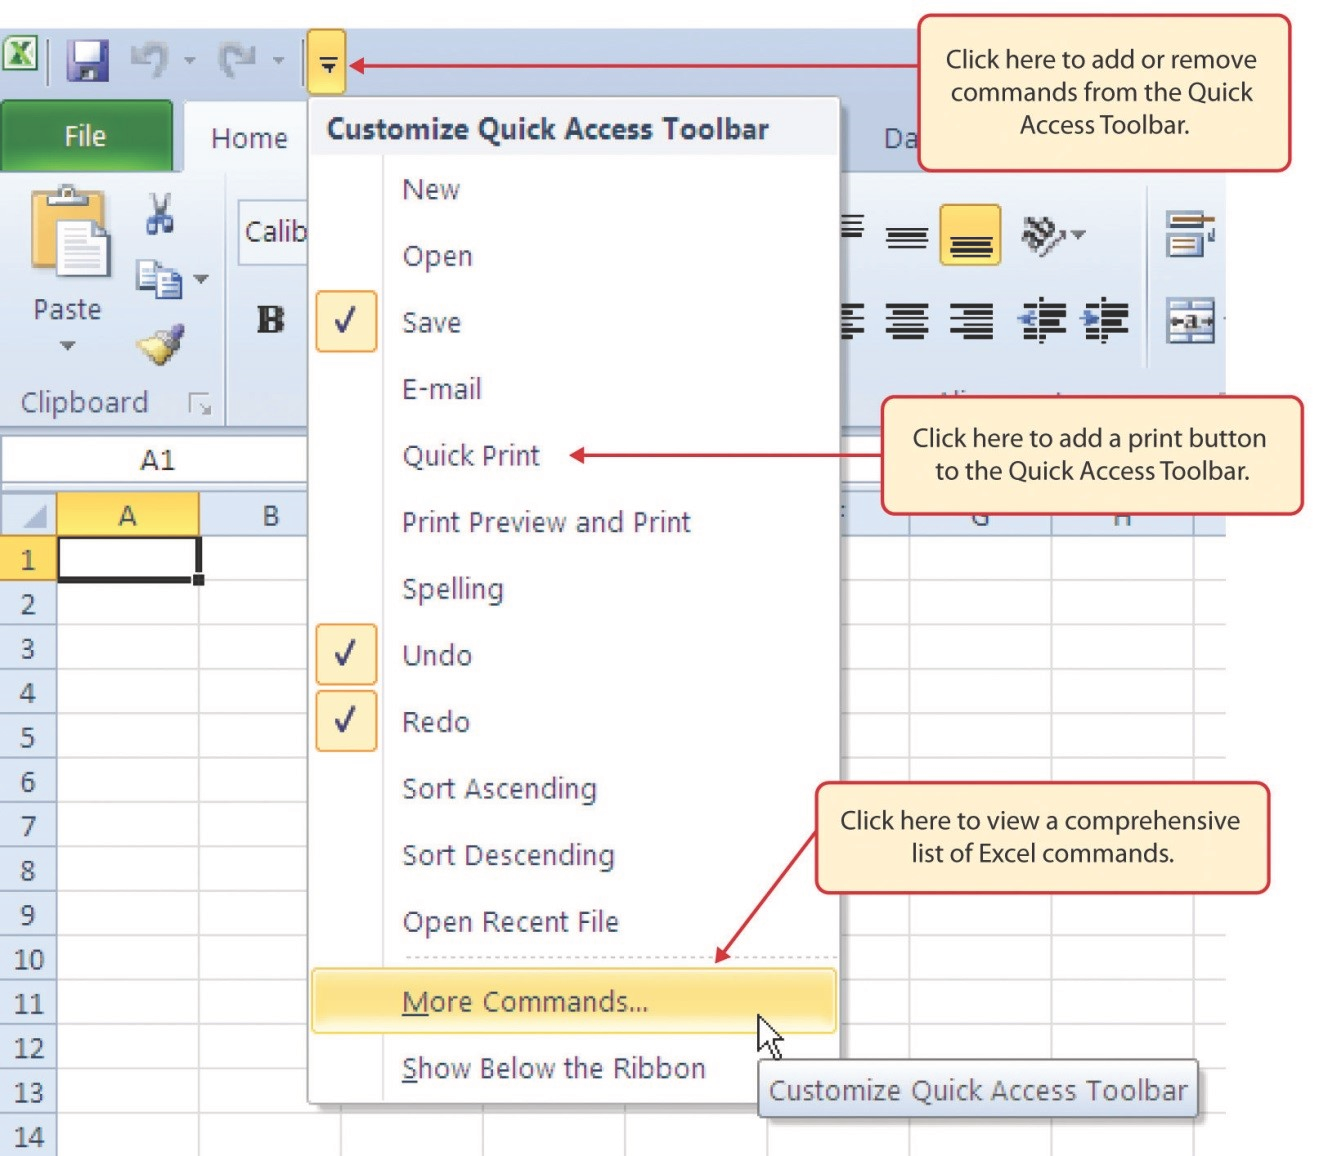
\includegraphics[width=\maxwidth{.95\linewidth}]{gfx/ch01_fig07}
	\caption{Customizing the Quick Access Toolbar}
	\label{01:fig07}
\end{figure}

In addition to the Ribbon and Quick Access Toolbar, you can also access commands by right clicking anywhere on the worksheet. \ref{01:fig08} shows an example of the commands available in the right-click menu.

\begin{figure}[H]
	\centering
	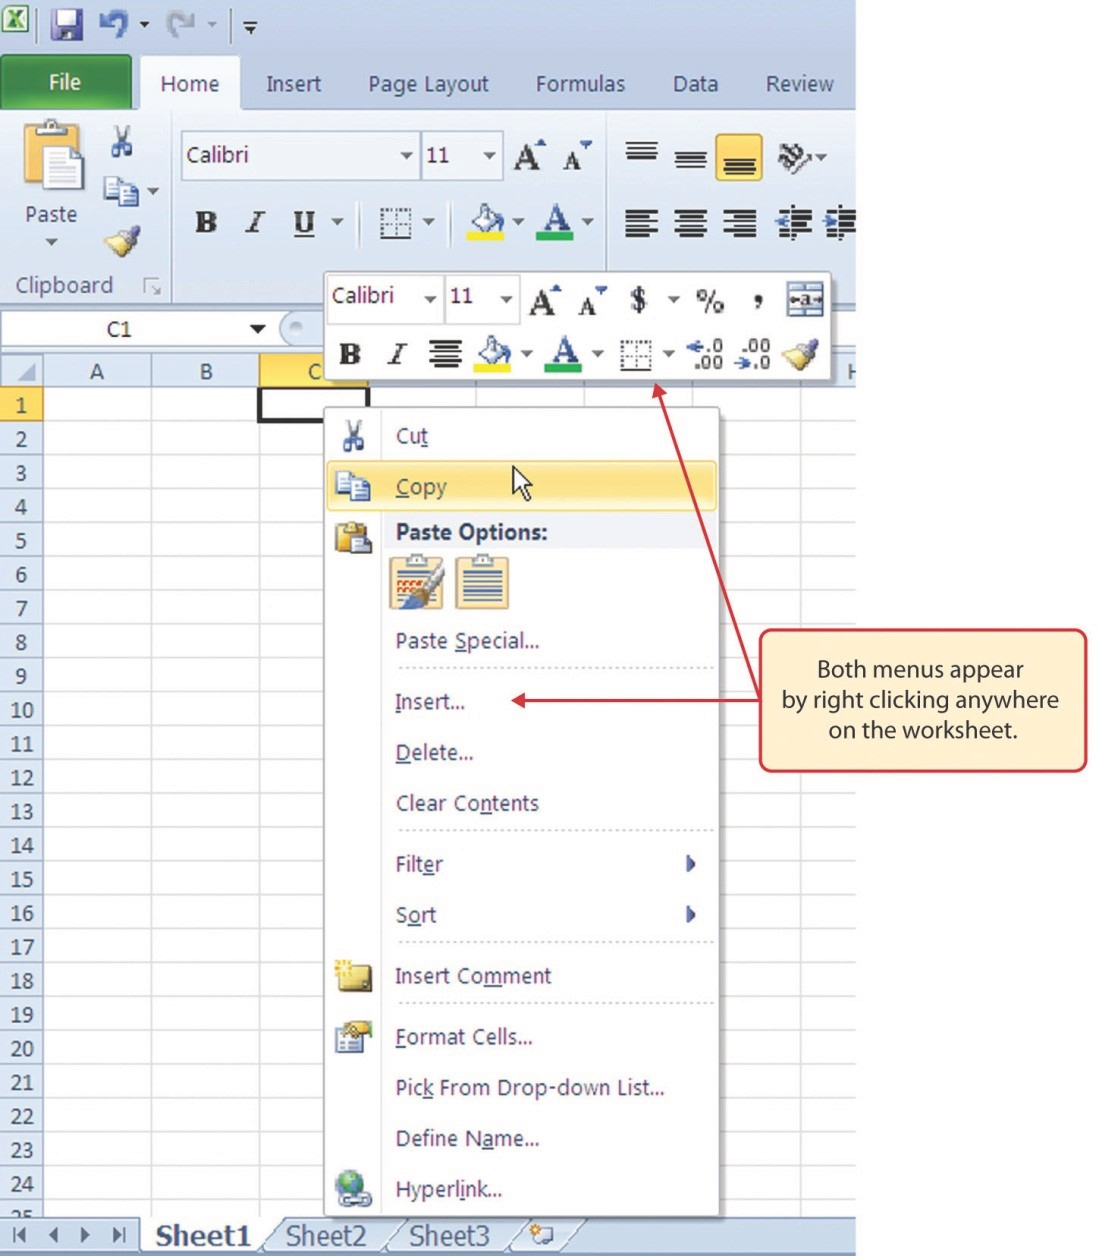
\includegraphics[width=\maxwidth{.95\linewidth}]{gfx/ch01_fig08}
	\caption{Right-Click Menu}
	\label{01:fig08}
\end{figure}

\subsection{The File Tab}

The File tab is also known as the Backstage view of the workbook. It contains a variety of features and commands related to the workbook that is currently open, new workbooks, or workbooks stored in other locations on your computer or network. Figure \ref{01:fig09} shows the options available in the File tab or Backstage view. To leave the Backstage view and return to the worksheet, click the arrow in the upper left-hand corner as shown below.

\begin{figure}[H]
	\centering
	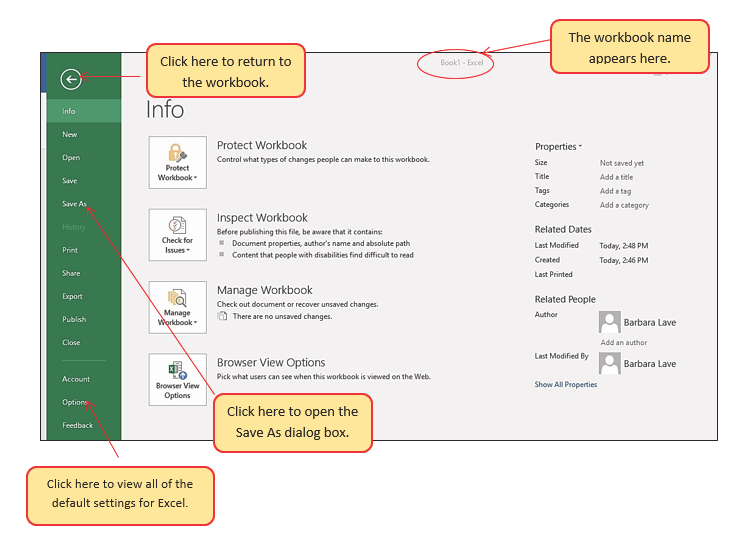
\includegraphics[width=\maxwidth{.95\linewidth}]{gfx/ch01_fig09}
	\caption{File Tab or Backstage View of a Workbook}
	\label{01:fig09}
\end{figure}

Included in the File tab are the default settings for the Excel application that can be accessed and modified by clicking the Options button. Figure \ref{01:fig10} shows the Excel Options window, which gives you access to settings such as the default font style, font size, and the number of worksheets that appear in new workbooks.

\begin{figure}[H]
	\centering
	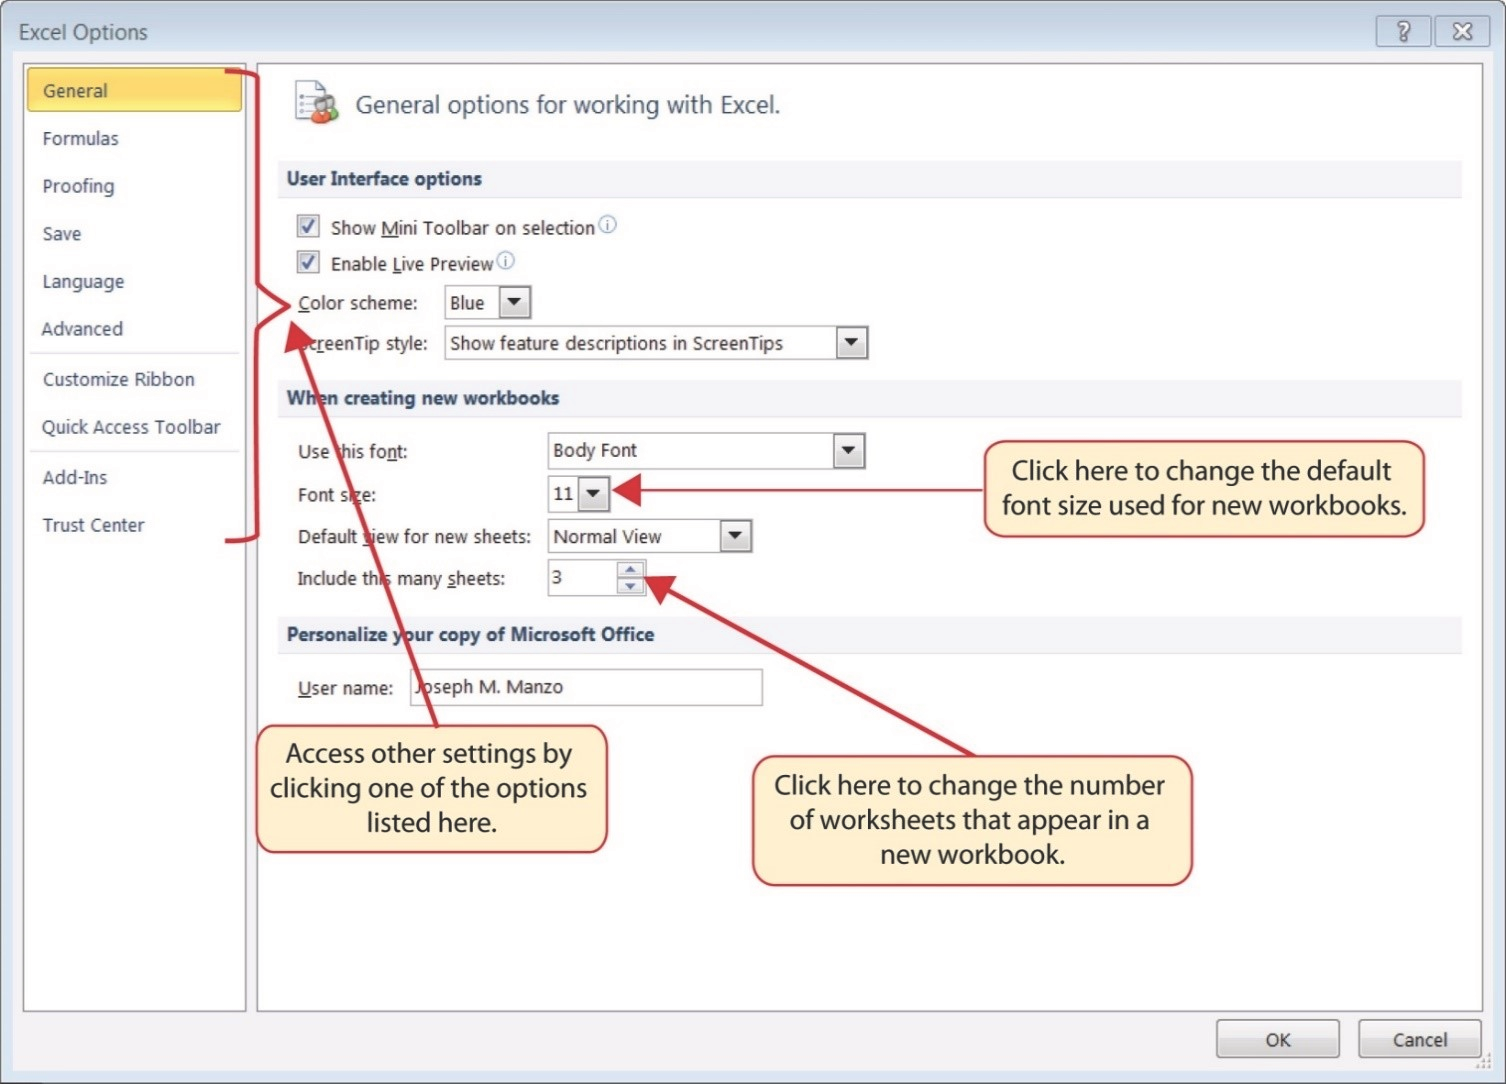
\includegraphics[width=\maxwidth{.95\linewidth}]{gfx/ch01_fig10}
	\caption{Excel Options Window}
	\label{01:fig10}
\end{figure}

\subsection{Saving Workbooks (Save As)}

Once you create a new workbook, you will need to change the file name and choose a location on your computer or network to save that file. It is important to remember where you save this workbook on your computer or network as you will be using this file in the Section 1.2 “Entering, Editing, and Managing Data” to construct the workbook shown in Figure \ref{01:fig01}. The process of saving can be different with different versions of Excel. Please be sure you follow the steps for the version of Excel you are using. The following steps explain how to save a new workbook and assign it a file name.

\subsubsection{Saving Workbooks in Excel 2013}

\begin{enumerate}
	\item If you have not done so already, open a blank workbook in Excel.
	\item When saving your workbook for the \textit{first} time, click the File tab.
	\item Click the Save As button in the upper left side of the Backstage view window. This will open the Save As dialog box, as shown in Figure \ref{01:fig11}.
	\item Click in the File Name box at the bottom of the Save As dialog box and use the \keystroke{Backspace} key to remove the current default name of the workbook.
	\item Type the file name: \textbf{CH1 GMW Sales Data}.
	\item Click the Desktop button on the left side of the Save As dialog box if you wish to save this file on your desktop. If you want to save this workbook in a different location, such as a USB drive, select your preferred location.
	\item Click the Save button on the lower right side of the Save As dialog box.
	\item As you continue to work on your workbook, you will want to Save frequently by click either the Save button on the Home ribbon or by selecting the Save option from the File menu.
\end{enumerate}

\begin{figure}[H]
	\centering
	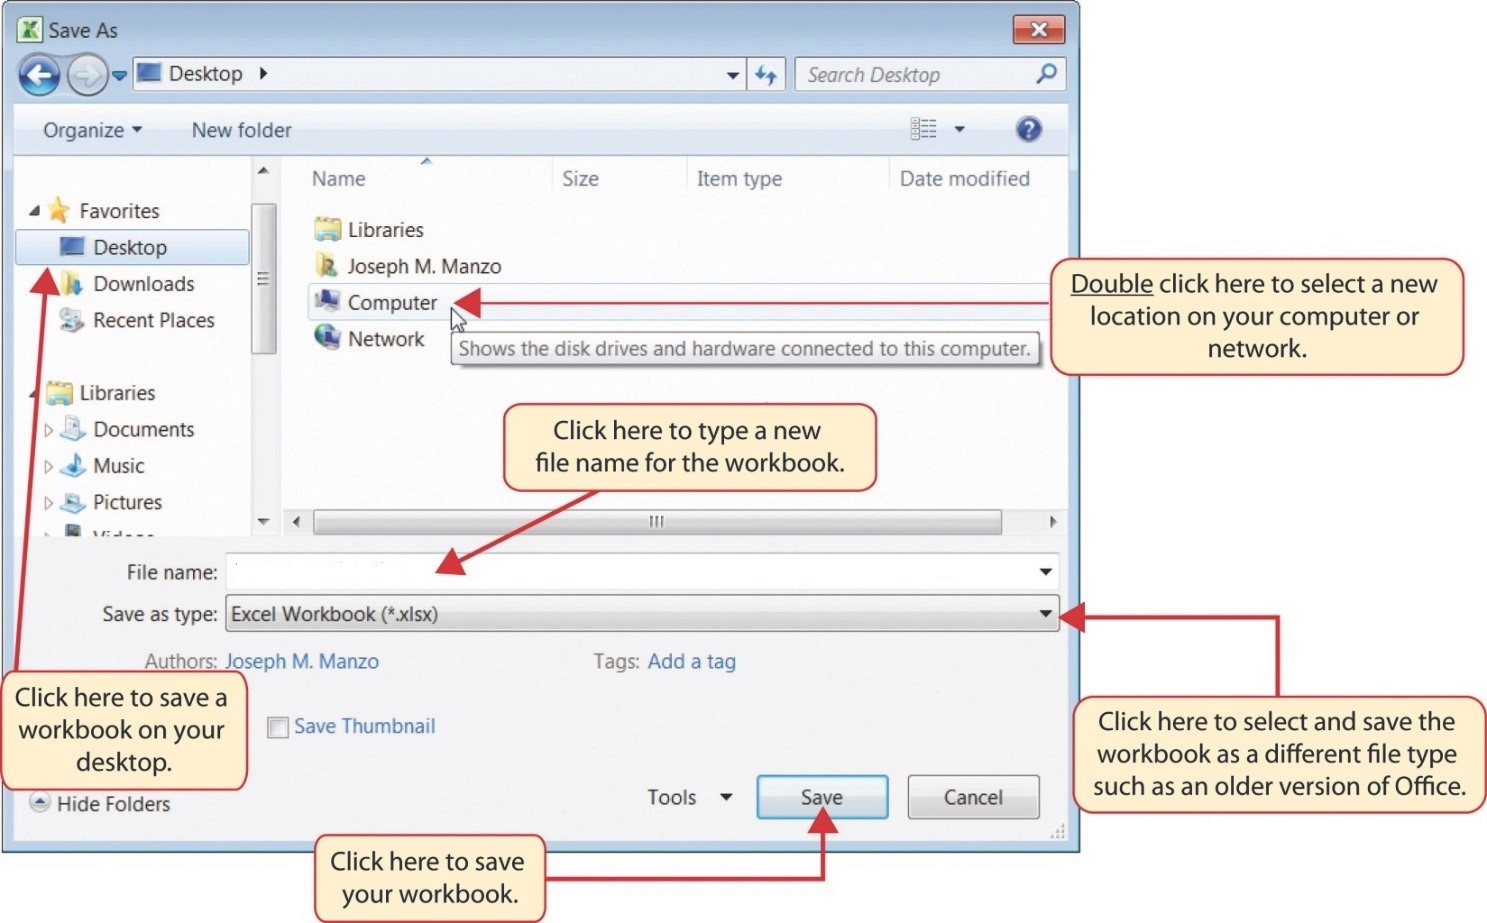
\includegraphics[width=\maxwidth{.95\linewidth}]{gfx/ch01_fig11}
	\caption{Save As Dialog Box in Excel 2013}
	\label{01:fig11}
\end{figure}

\subsubsection{Saving Workbooks in Excel 2016}

\begin{itemize}
	\item If you have not done so already, open a blank workbook in Excel.
	\item Click the File tab and then the Save As button in the left side of the Backstage view window. This will open the Save As dialog box.
	\item Determine a location for saving on your computer by clicking Browse on the left side to open the Save As dialog box as illustrated in Figure \ref{01:fig12}.
	\item Click in the File Name box near the bottom of the Save As dialog box. Type the new file name: \textbf{CH1 GMW Sales Data}
	\item Review the settings in the screen for correctness and click the Save button.
\end{itemize}

\begin{figure}[H]
	\centering
	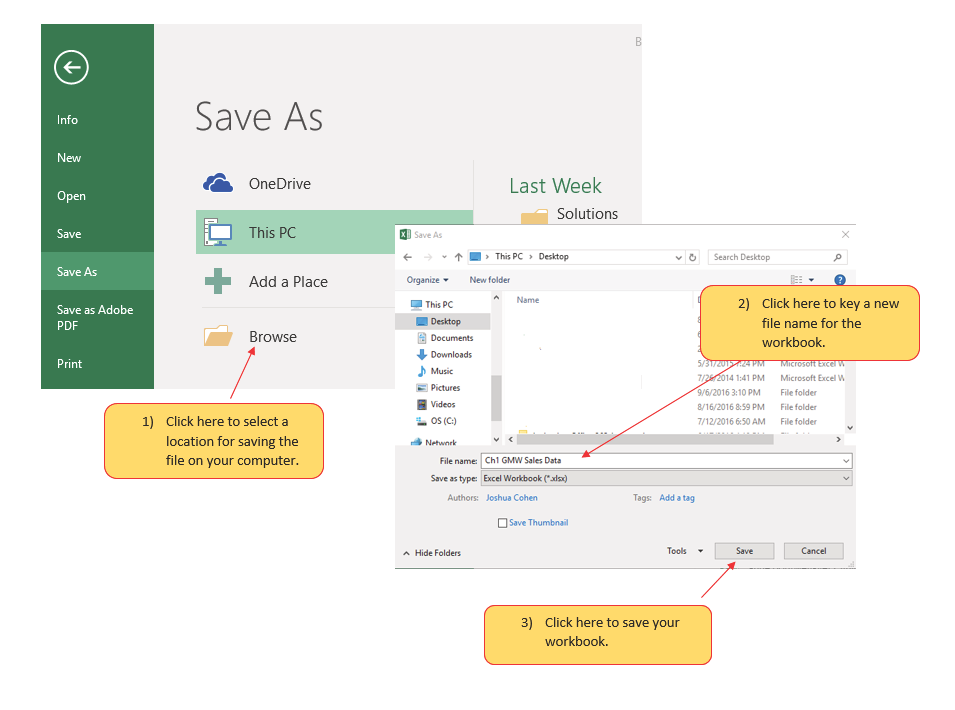
\includegraphics[width=\maxwidth{.95\linewidth}]{gfx/ch01_fig12}
	\caption{Save As Dialog in 2016}
	\label{01:fig12}
\end{figure}

\begin{center}
	\begin{shtcutbox}{Keyboard Shortcuts}
		\textbf{Save As}
		\\
		\begin{itemize}
			\setlength{\itemsep}{0pt}
			\setlength{\parskip}{0pt}
			\setlength{\parsep}{0pt}
			
			\item Press the \keystroke{F12} key and use the tab and arrow keys to navigate around the Save As dialog box. Use the \keystroke{Enter} key to make a selection.
			\item Or press the \keystroke{Alt} key on your keyboard. You will see letters and numbers, called Key Tips, appear on the Ribbon. Press the \keystroke{F} key on your keyboard for the File tab and then the \keystroke{A} key. This will open the Save As dialog box.
			
		\end{itemize}
	\end{shtcutbox}
\end{center}

\begin{center}
	\begin{sklbox}{Skill Refresher}
		\textbf{Saving Workbooks (Save As)}
		\\
		\begin{itemize}
			\setlength{\itemsep}{0pt}
			\setlength{\parskip}{0pt}
			\setlength{\parsep}{0pt}
			
			\item Click the File tab on the Ribbon.
			\item Click the Save As option.
			\item Select a location on your PC.
			\item Click in the File name box and type a new file name if needed.
			\item Click the down arrow next to the ``Save as type'' box and select the appropriate file type if needed.
			\item Click the Save button.
		
		\end{itemize}
	\end{sklbox}
\end{center}

\subsection{The Status Bar}

The Status Bar is located below the worksheet tabs on the Excel screen (see Figure \ref{01:fig13}). It displays a variety of information, such as the status of certain keys on your keyboard (e.g., CAPS LOCK), the available views for a workbook, the magnification of the screen, and mathematical functions that can be performed when data are highlighted on a worksheet. You can customize the Status Bar as follows:

\begin{enumerate}
	\item Place the mouse pointer over any area of the Status Bar and right click to display the ``Customize Status Bar'' list of options (see Figure \ref{01:fig13}).
	\item Select the Caps Lock option from the menu (see Figure \ref{01:fig13}).
	\item Press the \keystroke{Caps Lock} key on your keyboard. You will see the Caps Lock indicator on the lower right side of the Status Bar.
	\item Press the \keystroke{Caps Lock} on your keyboard again. The indicator on the Status Bar goes away.
\end{enumerate}

\begin{figure}[H]
	\centering
	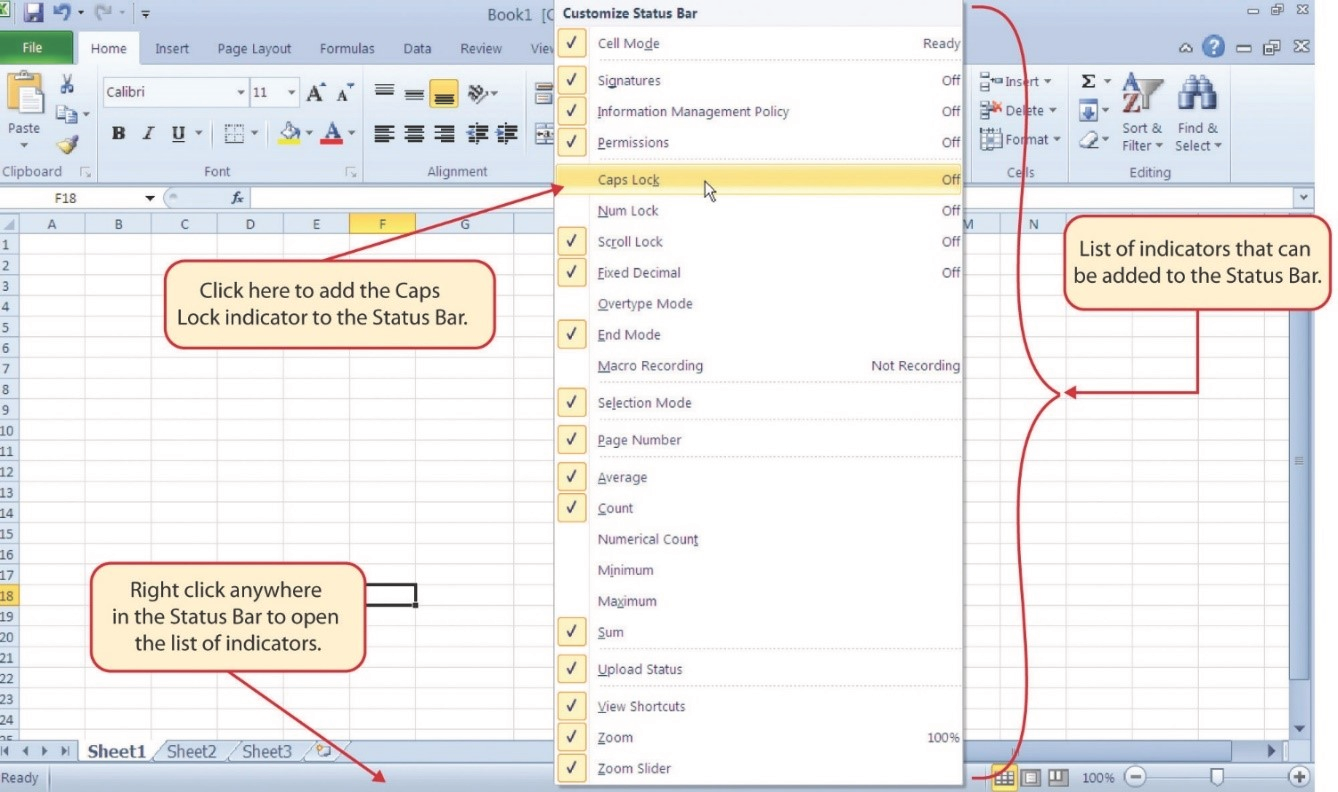
\includegraphics[width=\maxwidth{.95\linewidth}]{gfx/ch01_fig13}
	\caption{Customizing the Status Bar}
	\label{01:fig13}
\end{figure}

\subsection{Excel Help}

The Help feature provides extensive information about the Excel application. Although some of this information may be stored on your computer, the Help window will automatically connect to the Internet, if you have a live connection, to provide you with resources that can answer most of your questions. You can open the Excel Help window by clicking the question mark in the upper right area of the screen or ribbon. With newer versions of Excel, use the query box to enter your question and select from helpful option links or select the question mark from the dropdown list to launch Excel Help windows.

\begin{figure}[H]
	\centering
	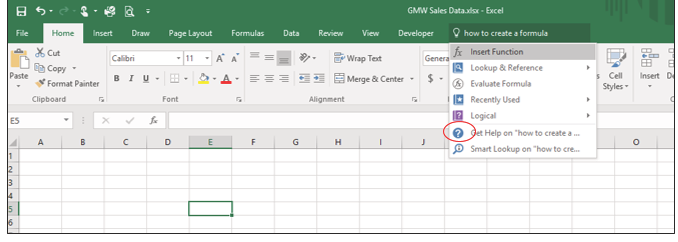
\includegraphics[width=\maxwidth{.95\linewidth}]{gfx/ch01_fig14}
	\caption{Excel Help Window}
	\label{01:fig14}
\end{figure}

\begin{center}
	\begin{shtcutbox}{Keyboard Shortcuts}
		\textbf{Excel Help}
		\\
		\begin{itemize}
			\setlength{\itemsep}{0pt}
			\setlength{\parskip}{0pt}
			\setlength{\parsep}{0pt}
			
			\item Press the \keystroke{F1} key on your keyboard.
			
		\end{itemize}
	\end{shtcutbox}
\end{center}


\begin{center}
	\begin{tkwbox}{Key Take-Aways}
		\textbf{Overview}
		\\
		\begin{itemize}
			\setlength{\itemsep}{0pt}
			\setlength{\parskip}{0pt}
			\setlength{\parsep}{0pt}
			
			\item Excel is a powerful tool for processing data for the purposes of making decisions.
			\item You can find Excel commands throughout the tabs in the Ribbon.
			\item You can customize the Quick Access Toolbar by adding commands you frequently use.
			\item You can add or remove the information that is displayed on the Status Bar.
			\item The Help window provides you with extensive information about Excel.
			
		\end{itemize}
	\end{tkwbox}
\end{center}

\section{Entering, Editing, and Managing Data}

\begin{center}
	\begin{objbox}{Learning Objectives}
		\begin{itemize}
			\setlength{\itemsep}{0pt}
			\setlength{\parskip}{0pt}
			\setlength{\parsep}{0pt}
			
			\item Understand how to enter data into a worksheet.
			\item Examine how to edit data in a worksheet.
			\item Examine how Auto Fill is used when entering data.
			\item Understand how to delete data from a worksheet and use the Undo command.
			\item Examine how to adjust column widths and row heights in a worksheet.
			\item Understand how to hide columns and rows in a worksheet.
			\item Examine how to insert columns and rows into a worksheet.
			\item Understand how to delete columns and rows from a worksheet.
			\item Learn how to move data to different locations in a worksheet.

		\end{itemize}
	\end{objbox}
\end{center}

In this section, we will begin the development of the workbook shown in Figure \ref{01:fig01}. The skills covered in this section are typically used in the early stages of developing one or more worksheets in a workbook.

\subsection{Entering Data}

You will begin building the workbook shown in Figure \ref{01:fig01} by manually entering data into the worksheet. The following steps explain how the column headings in Row 2 are typed into the worksheet:

\begin{enumerate}
	\item Click cell location \textsf{A2} on the worksheet.
	\item Type the word \textbf{Month}.
	\item Press the \keystroke{Right Arrow} key. This will enter the word into cell \textsf{A2} and activate the next cell to the right.
	\item Type \textbf{Unit Sales} and press the \keystroke{Right Arrow} key.
	\item Repeat step 4 for the words \textbf{Average Price} and then again for \textbf{Sales Dollars}.
\end{enumerate}

Figure \ref{01:fig15} shows how your worksheet should appear after you have typed the column headings into Row 2. Notice that the word \textbf{Price} in cell location \textsf{C2} is not visible. This is because the column is too narrow to fit the entry you typed. We will examine formatting techniques to correct this problem in the next section.

\begin{figure}[H]
	\centering
	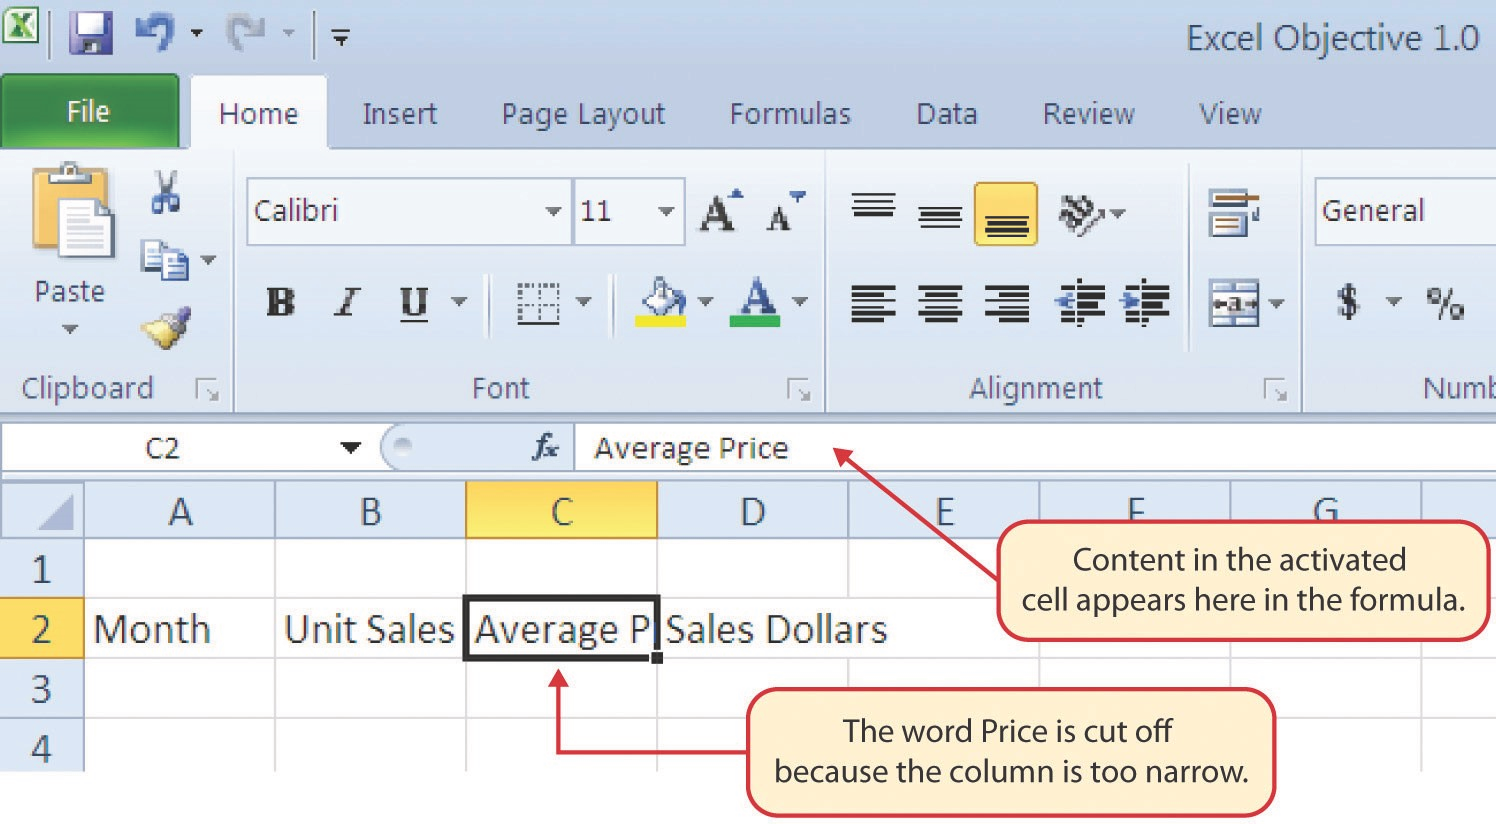
\includegraphics[width=\maxwidth{.95\linewidth}]{gfx/ch01_fig15}
	\caption{Entering Column Headings into a Worksheet}
	\label{01:fig15}
\end{figure}

\begin{enumerate}
	\item Click cell location \textsf{B3}.
	\item Type the number \textbf{2670} and press the \keystroke{Enter} key. After you press the \keystroke{Enter} key, cell \textsf{B4} will be activated. Using the \keystroke{Enter} key is an efficient way to enter data vertically down a column.
	\item Enter the following numbers in cells \textsf{B4} through \textsf{B14}: \textbf{2160}, \textbf{515}, \textbf{590}, \textbf{1030}, \textbf{2875}, \textbf{2700}, \textbf{900}, \textbf{775}, \textbf{1180}, \textbf{1800}, and \textbf{3560}.
	\item Click cell location \textsf{C3}.
	\item Type the number \textbf{9.99} and press the \keystroke{Enter} key.
	\item Enter the following numbers in cells \textsf{C4} through \textsf{C14}: \textbf{12.49}, \textbf{14.99}, \textbf{17.49}, \textbf{14.99}, \textbf{12.49}, \textbf{9.99}, \textbf{19.99}, \textbf{19.99}, \textbf{19.99}, \textbf{17.49}, and \textbf{14.99}.
	\item Activate cell location \textsf{D3}.
	\item Type the number \textbf{26685} and press the \keystroke{Enter} key.
	\item Enter the following numbers in cells \textsf{D4} through \textsf{D14}: \textbf{26937}, \textbf{7701}, \textbf{10269}, \textbf{15405}, \textbf{35916}, \textbf{26937}, \textbf{17958}, \textbf{15708}, \textbf{23562}, \textbf{31416}, and \textbf{53370}.
	\item When finished, check that the data you entered matches Figure \ref{01:fig16}.
\end{enumerate}

\begin{center}
	\begin{infobox}{Integrity Check}
		\textbf{Column Headings}
		\\
		\\
		It is critical to include column headings that accurately describe the data in each column of a worksheet. In professional environments, you will likely be sharing Excel workbooks with coworkers. Good column headings reduce the chance of someone misinterpreting the data contained in a worksheet, which could lead to costly errors depending on your career.
	\end{infobox}
\end{center}

\begin{figure}[H]
	\centering
	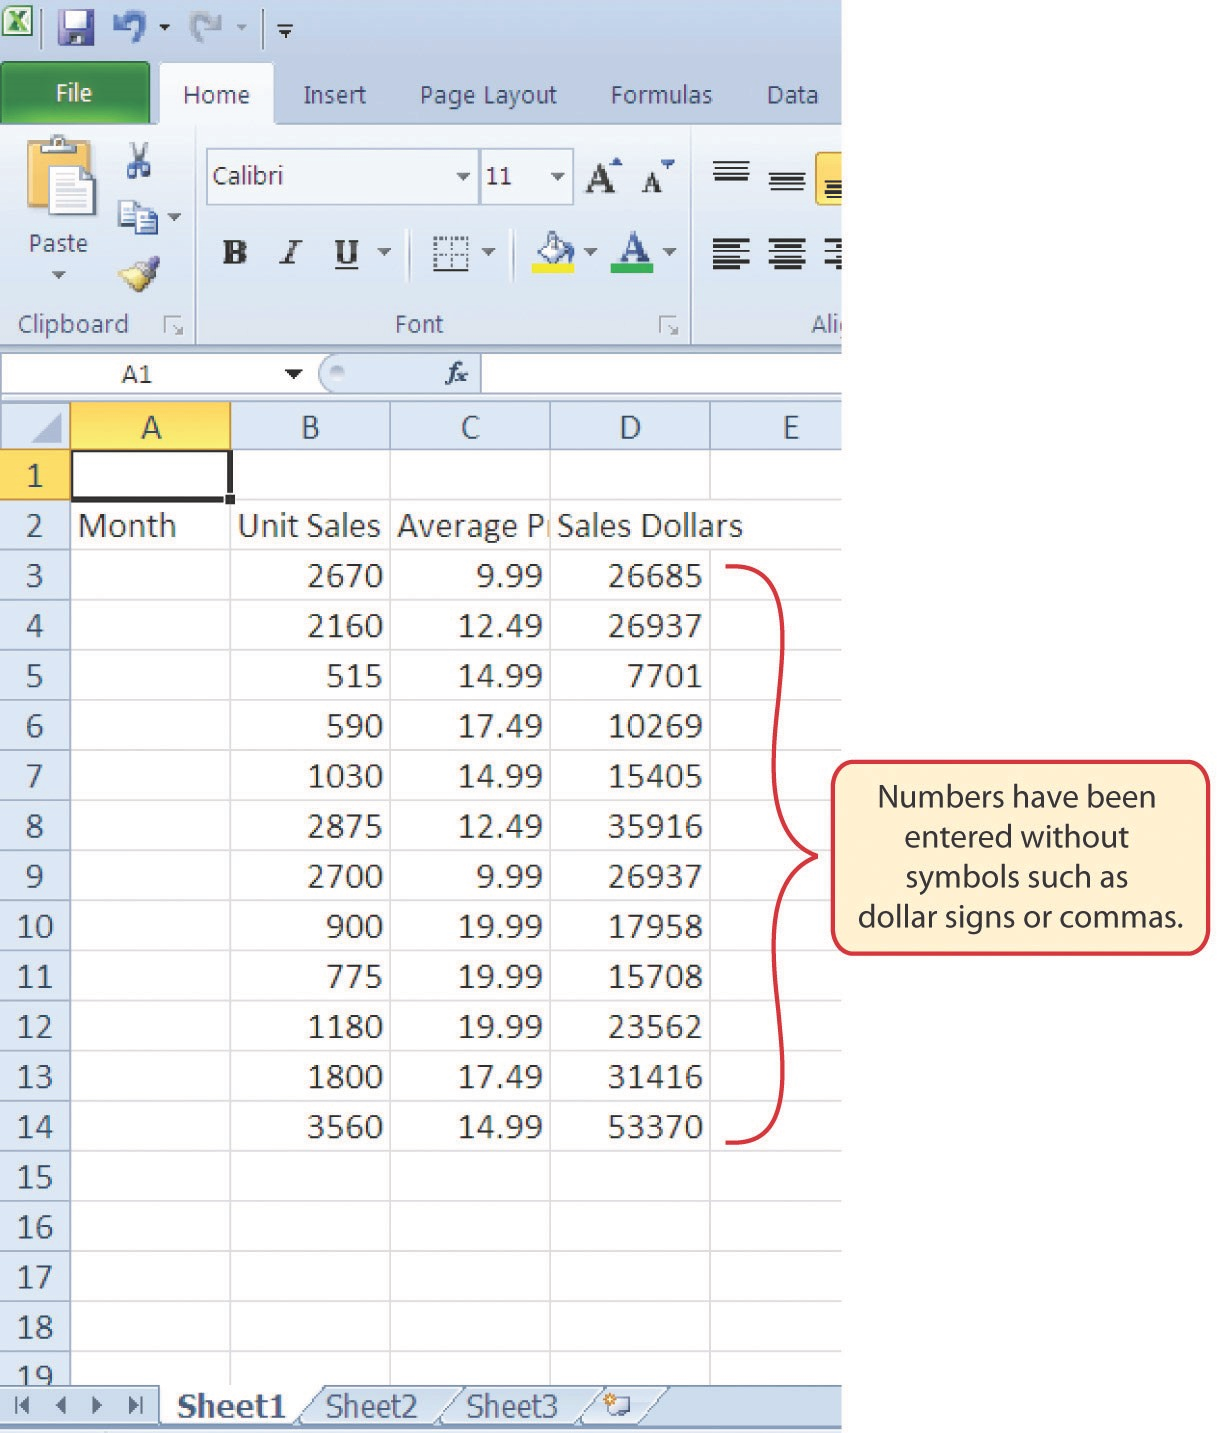
\includegraphics[width=\maxwidth{.95\linewidth}]{gfx/ch01_fig16}
	\caption{Completed Data Entry for Columns B, C, and D}
	\label{01:fig16}
\end{figure}

\subsection{Editing Data}

Data that has been entered in a cell can be changed by double clicking the cell location or using the Formula Bar. You may have noticed that as you were typing data into a cell location, the data you typed appeared in the Formula Bar. The Formula Bar can be used for entering data into cells as well as for editing data that already exists in a cell. The following steps provide an example of entering and then editing data that has been entered into a cell location:

\begin{enumerate}
	\item Click cell \textsf{A15} in the Sheet1 worksheet.
	\item Type the abbreviation \textbf{Tot} and press the \keystroke{Enter} key.
	\item Click cell \textsf{A15}.
	\item Move the mouse pointer up to the Formula Bar. You will see the pointer turn into a cursor. Move the cursor to the end of the abbreviation \textbf{Tot} and left click.
	\item Type the letters \textbf{al} to complete the word ``Total.''
\end{enumerate}

\begin{center}
	\begin{infobox}{Why?}
		\textbf{Avoid Formatting Symbols When Entering Numbers}
		\\
		\\
		When typing numbers into an Excel worksheet, it is best to avoid adding any formatting symbols such as dollar signs and commas. Although Excel allows you to add these symbols while typing numbers, it slows down the process of entering data. It is more efficient to use Excel's formatting features to add these symbols to numbers after you type them into a worksheet.
	\end{infobox}
\end{center}

\begin{center}
	\begin{infobox}{Integrity Check}
		\textbf{Data Entry}
		\\
		\\
		It is very important to proofread your worksheet carefully, especially when you have entered numbers. Transposing numbers when entering data manually into a worksheet is a common error. For example, the number 563 could be transposed to 536. Such errors can seriously compromise the integrity of your workbook.
	\end{infobox}
\end{center}


\begin{enumerate}[resume]
	\item Click the checkmark to the left of the Formula Bar (see Figure \ref{01:fig17}). This will enter the change into the cell.
\end{enumerate}

\begin{figure}[H]
	\centering
	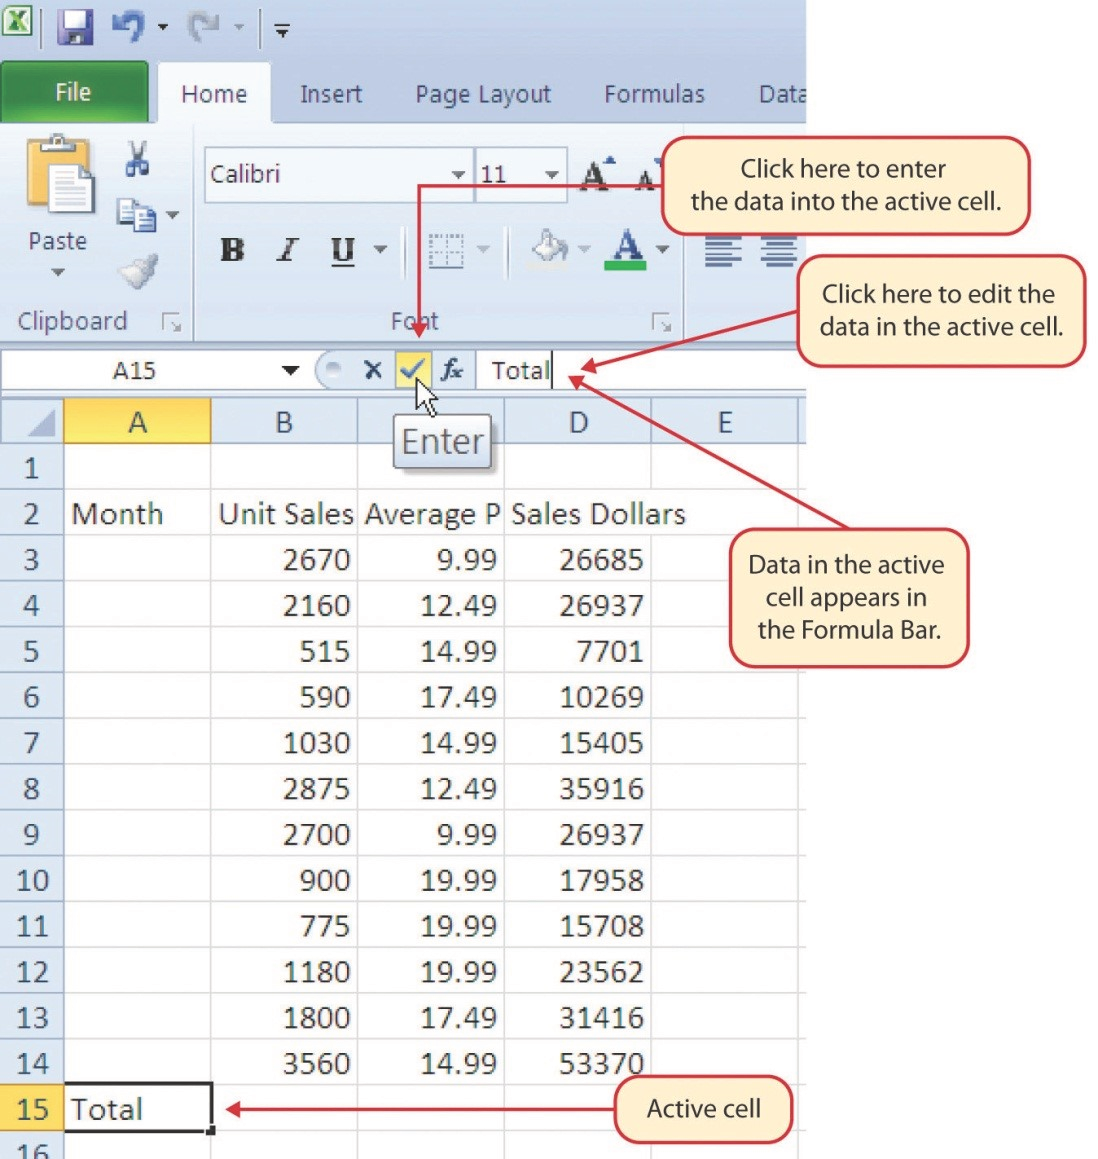
\includegraphics[width=\maxwidth{.95\linewidth}]{gfx/ch01_fig17}
	\caption{Using the Formula Bar to Edit and Enter Data}
	\label{01:fig17}
\end{figure}

\begin{enumerate}[resume]
	\item Double click cell \textsf{A15}.
	\item Add a space after the word Total and type the word \textbf{Sales}.
	\item Press the \keystroke{Enter} key.
\end{enumerate}

\begin{center}
	\begin{shtcutbox}{Keyboard Shortcuts}
		\textbf{Editing Data in a Cell}
		\\
		\begin{itemize}
			\setlength{\itemsep}{0pt}
			\setlength{\parskip}{0pt}
			\setlength{\parsep}{0pt}
			
			\item Activate the cell that is to be edited and press the \keystroke{F2} key on your keyboard.
			
		\end{itemize}
	\end{shtcutbox}
\end{center}

\subsection{Auto Fill}

The Auto Fill feature is a valuable tool when manually entering data into a worksheet. This feature has many uses, but it is most beneficial when you are entering data in a defined sequence, such as the numbers 2, 4, 6, 8, and so on, or non-numeric data such as the days of the week or months of the year. The following steps demonstrate how Auto Fill can be used to enter the months of the year in Column A:

\begin{enumerate}
	\item Click cell \textsf{A3} in the Sheet1 worksheet.
	\item Type the word \textbf{January} and press the \keystroke{Enter} key.
	\item Activate cell \textsf{A3} again.
	\item Move the mouse pointer to the lower right corner of cell \textsf{A3}. You will see a small square in this corner of the cell; this is called the Fill Handle (See Figure \ref{01:fig18}) When the mouse pointer gets close to the Fill Handle, the white block plus sign will turn into a black plus sign.
\end{enumerate}

\begin{figure}[H]
	\centering
	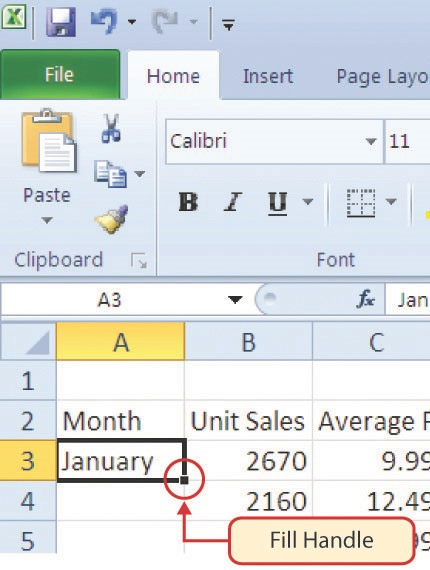
\includegraphics[width=\maxwidth{.95\linewidth}]{gfx/ch01_fig18}
	\caption{Fill Handle}
	\label{01:fig18}
\end{figure}

Left click and drag the Fill Handle to cell \textsf{A14}. Notice that the Auto Fill tip box indicates what month will be placed into each cell (see Figure \ref{01:fig19}). Release the left mouse button when the tip box reads ``December.''

\begin{figure}[H]
	\centering
	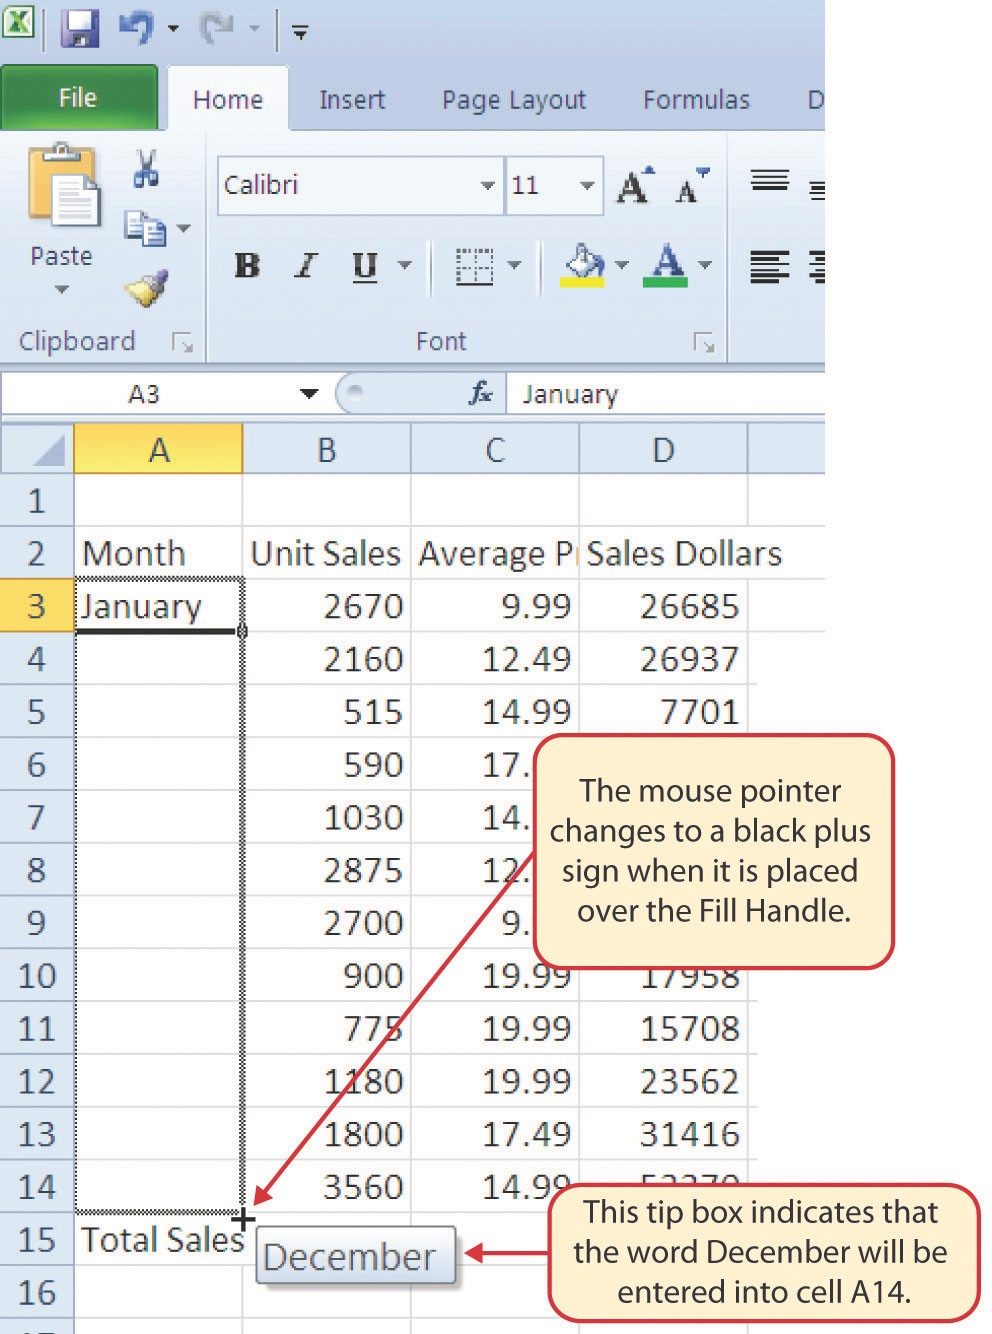
\includegraphics[width=\maxwidth{.95\linewidth}]{gfx/ch01_fig19}
	\caption{Using Auto Fill to Enter the Months of the Year}
	\label{01:fig19}
\end{figure}

Once you release the left mouse button, all twelve months of the year should appear in the cell range \textsf{A3:A14}, as shown in Figure \ref{01:fig20}. You will also see the Auto Fill Options button. By clicking this button, you have several options for inserting data into a group of cells.

\begin{figure}[H]
	\centering
	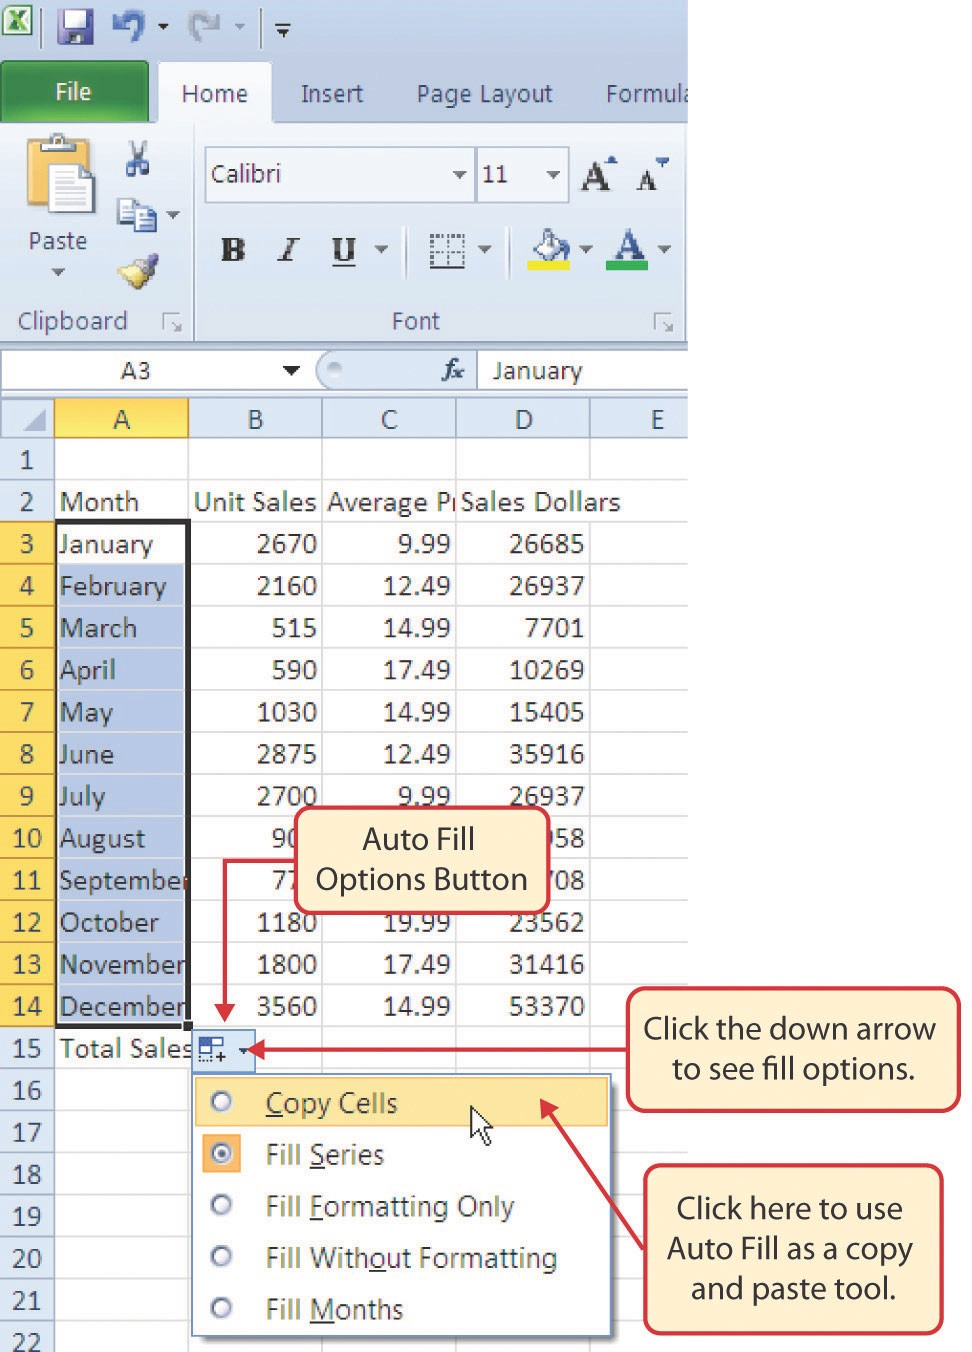
\includegraphics[width=\maxwidth{.95\linewidth}]{gfx/ch01_fig20}
	\caption{Auto Fill Options Button}
	\label{01:fig20}
\end{figure}

\begin{enumerate}
	\item Click the Auto Fill Options button.
	\item Click the Copy Cells option. This will change the months in the range \textsf{A4:A14} to January.
	\item Click the Auto Fill Options button again.
	\item Click the Fill Months option to return the months of the year to the cell range \textsf{A4:A14}. The Fill Series option will provide the same result.
\end{enumerate}

\subsection{Deleting Data and the Undo Command}

There are several methods for removing data from a worksheet, a few of which are demonstrated here. With each method, you use the Undo command. This is a helpful command in the event you mistakenly remove data from your worksheet. The following steps demonstrate how you can delete data from a cell or range of cells:

\begin{enumerate}
	\item Click cell \textsf{C2} by placing the mouse pointer over the cell and clicking the left mouse button.
	\item Press the \keystroke{Delete} key on your keyboard. This removes the contents of the cell.
	\item Highlight the range \textsf{C3:C14} by placing the mouse pointer over cell \textsf{C3} then left click and drag the mouse pointer down to cell \textsf{C14}.
	\item Place the mouse pointer over the Fill Handle. You will see the white block plus sign change to a black plus sign.
	\item Click and drag the mouse pointer up to cell \textsf{C3} (see Figure \ref{01:fig21}). Release the mouse button. The contents in the range \textsf{C3:C14} will be removed.
\end{enumerate}

\begin{figure}[H]
	\centering
	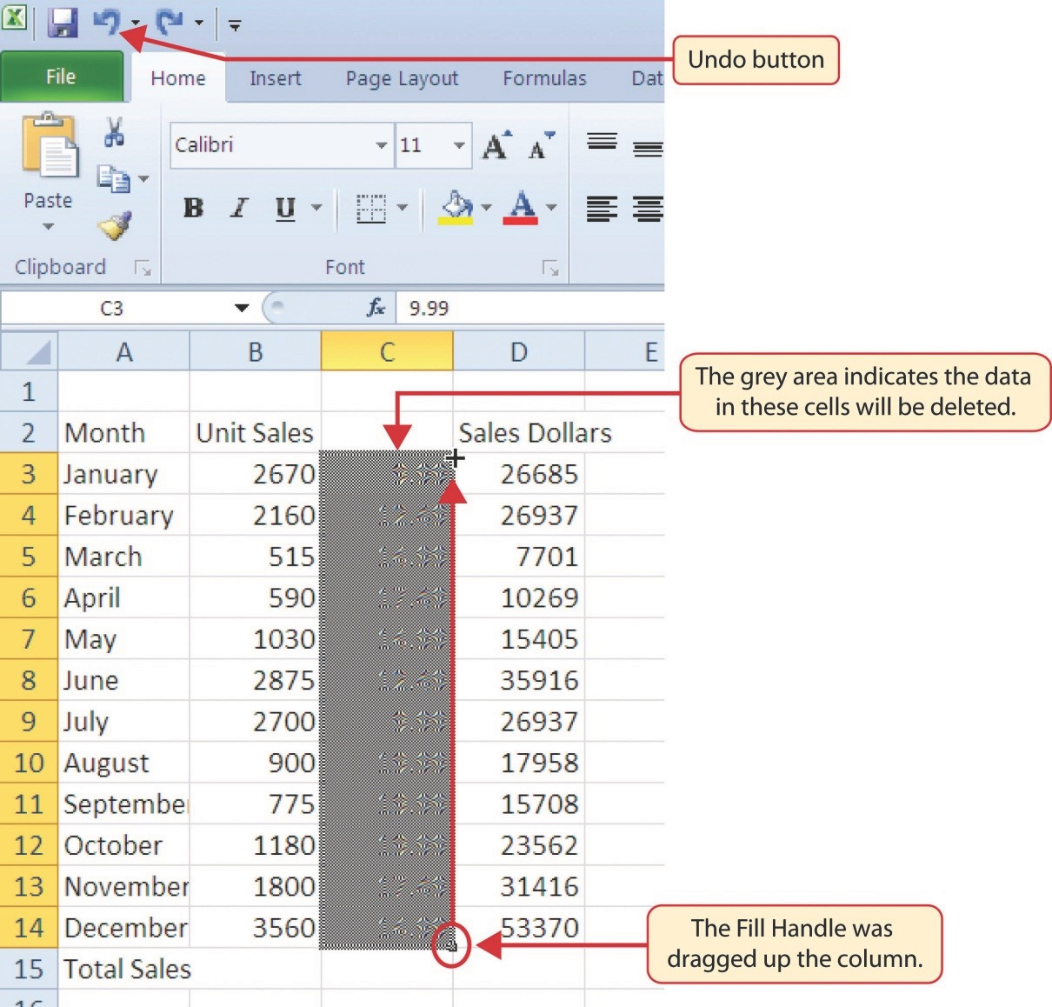
\includegraphics[width=\maxwidth{.95\linewidth}]{gfx/ch01_fig21}
	\caption{Using Auto Fill to Delete Contents of Cell}
	\label{01:fig21}
\end{figure}

\begin{enumerate}
	\item Click the Undo button in the Quick Access Toolbar (see Figure \ref{01:fig21}). This should replace the data in the range \textsf{C3:C14}.
	\item Click the Undo button again. This should replace the data in cell \textsf{C2}.
\end{enumerate}

\begin{center}
	\begin{shtcutbox}{Keyboard Shortcuts}
		\textbf{Undo Command}
		\\
		\begin{itemize}
			\setlength{\itemsep}{0pt}
			\setlength{\parskip}{0pt}
			\setlength{\parsep}{0pt}
			
			\item Hold down the \keystroke{Ctrl} key while pressing the letter \keystroke{Z} on your keyboard.
			
		\end{itemize}
	\end{shtcutbox}
\end{center}

\begin{enumerate}[resume]
	\item Highlight the range \textsf{C2:C14} by placing the mouse pointer over cell \textsf{C2}. Then left click and drag the mouse pointer down to cell \textsf{C14}.
	\item Click the Clear button in the Home tab of the Ribbon, which is next to the Cells group of commands (see Figure \ref{01:fig22}). This opens a drop-down menu that contains several options for removing or clearing data from a cell. Notice that you also have options for clearing just the formats or the hyperlinks in a cell.
	\item Click the Clear All option. This removes the data in the cell range.
	\item Click the Undo button. This replaces the data in the range \textsf{C2:C14}.
\end{enumerate}

\begin{figure}[H]
	\centering
	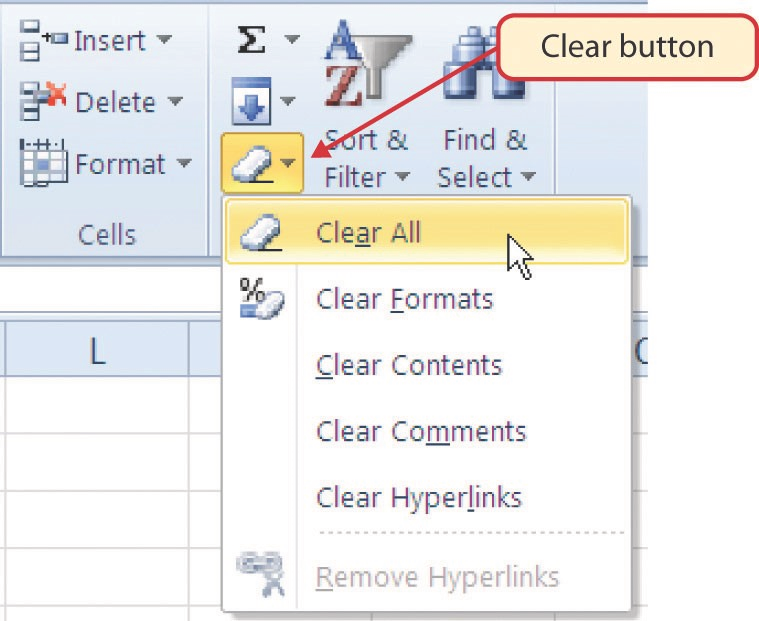
\includegraphics[width=\maxwidth{.95\linewidth}]{gfx/ch01_fig22}
	\caption{Clear Command Drop-Down Menu}
	\label{01:fig22}
\end{figure}

\subsection{Adjusting Columns and Rows}

There are a few entries in the worksheet that appear cut off. For example, the last letter of the word September cannot be seen in cell \textsf{A11}. This is because the column is too narrow for this word. The columns and rows on an Excel worksheet can be adjusted to accommodate the data that is being entered into a cell. The following steps explain how to adjust the column widths and row heights in a worksheet:

\begin{enumerate}
	\item Bring the mouse pointer between Column A and Column B in the Sheet1 worksheet, as shown in Figure \ref{01:fig23}. You will see the white block plus sign turn into double arrows.
	\item Click and drag the column to the right so the entire word September in cell \textsf{A11} can be seen. As you drag the column, you will see the column width tip box. This box displays the number of characters that will fit into the column using the Calibri 11-point font which is the default setting for font/size.
	\item Release the left mouse button.
\end{enumerate}

\begin{figure}[H]
	\centering
	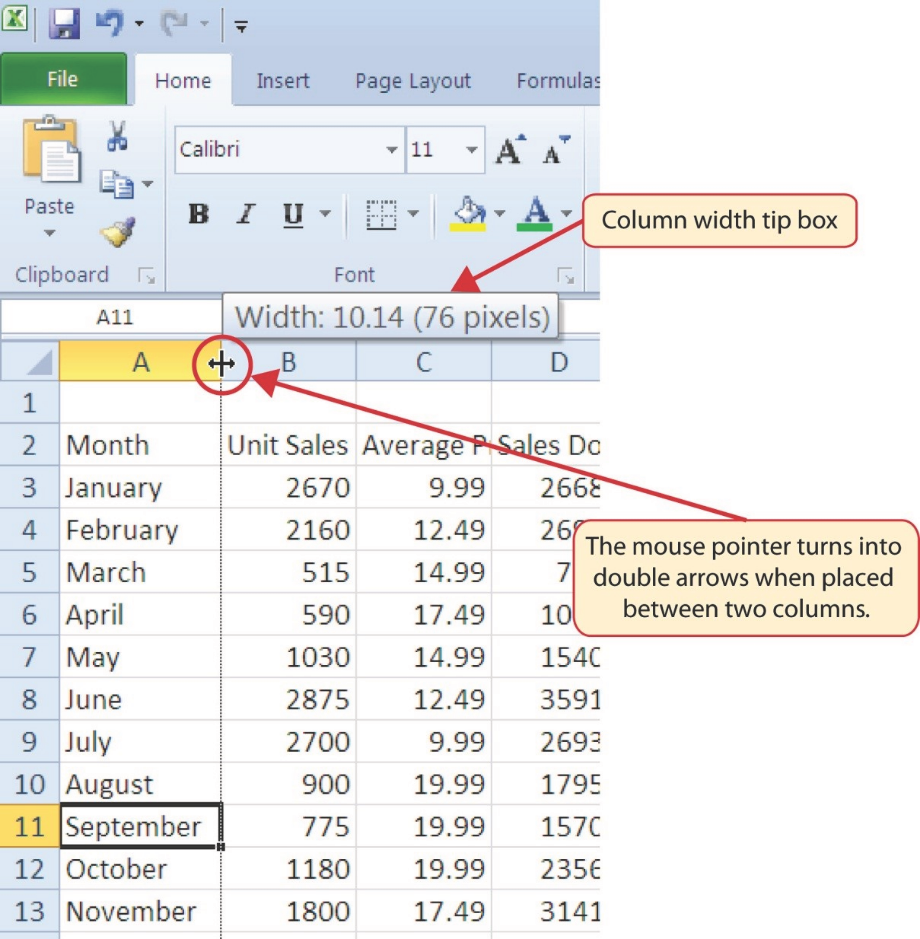
\includegraphics[width=\maxwidth{.95\linewidth}]{gfx/ch01_fig23}
	\caption{Adjusting Column Widths}
	\label{01:fig23}
\end{figure}

You may find that using the click-and-drag method is inefficient if you need to set a specific character width for one or more columns. The following steps illustrate a second method for adjusting column widths when using a specific number of characters.

\begin{enumerate}
	\item Click any cell location in Column \textsf{A} by moving the mouse pointer over a cell location and clicking the left mouse button. You can highlight cell locations in multiple columns if you are setting the same character width for more than one column.
	\item In the Home tab of the Ribbon, left click the Format button in the Cells group.
	\item Click the Column Width option from the drop-down menu. This will open the Column Width dialog box.
	\item Type the number \textbf{13} and click the OK button on the Column Width dialog box. This will set Column \textsf{A} to this character width (see Figure \ref{01:fig24}).
	\item Once again bring the mouse pointer between Column \textsf{A} and Column \textsf{B} so that the double arrow pointer displays and then double-click to activate AutoFit. This features adjusts the column width based on the longest entry in the column.
	\item Use the Column Width dialog box to reset the width to \textbf{13}.
\end{enumerate}

\begin{figure}[H]
	\centering
	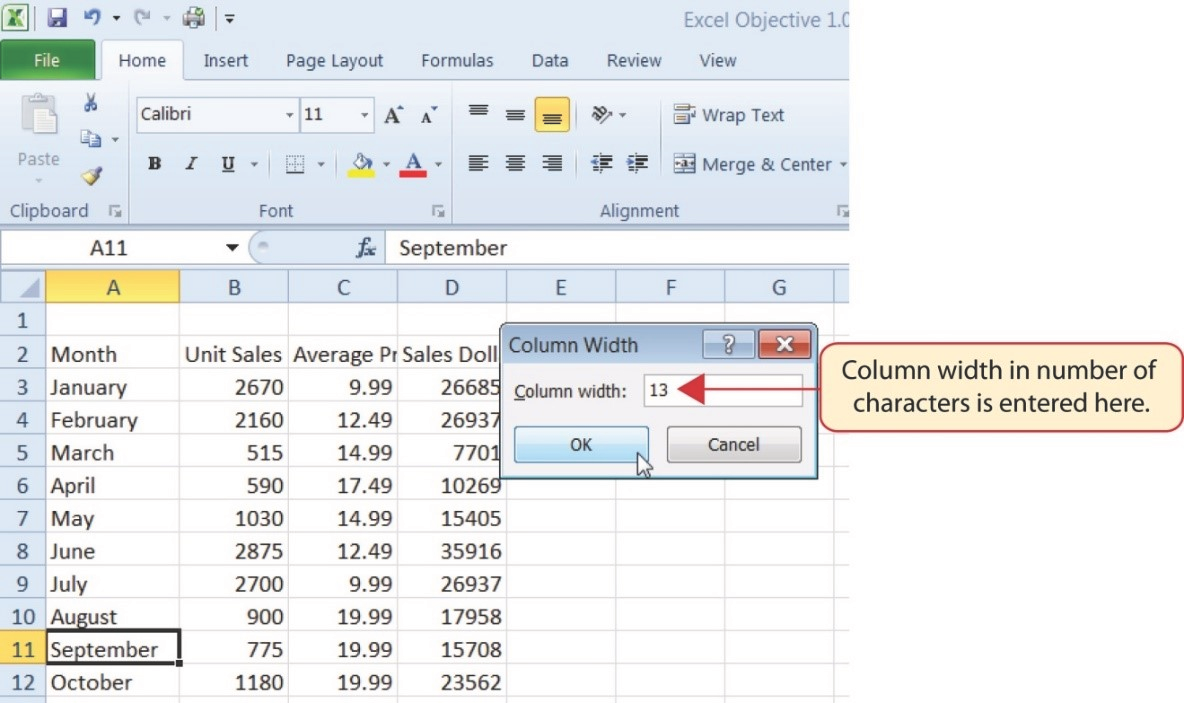
\includegraphics[width=\maxwidth{.95\linewidth}]{gfx/ch01_fig24}
	\caption{Column Width Dialog Box}
	\label{01:fig24}
\end{figure}

\begin{center}
	\begin{shtcutbox}{Keyboard Shortcuts}
		\textbf{Column Width}
		\\
		\begin{itemize}
			\setlength{\itemsep}{0pt}
			\setlength{\parskip}{0pt}
			\setlength{\parsep}{0pt}
			
			\item Press the \keystroke{Alt} key on your keyboard, then press the letters \keystroke{H}, \keystroke{O}, and \keystroke{W} one at a time.
			
		\end{itemize}
	\end{shtcutbox}
\end{center}

The following steps demonstrate how to adjust row height, which is similar to adjusting column width.

\begin{enumerate}
	\item Click cell \textsf{A15} by placing the mouse pointer over the cell and clicking the left mouse button.
	\item In the Home tab of the Ribbon, left click the Format button in the Cells group.
	\item Click the Row Height option from the drop-down menu. This will open the Row Height dialog box.
	\item Type the number \textbf{24} and click the OK button on the Row Height dialog box. This will set Row 15 to a height of 24 points. A point is equivalent to approximately 1/72 of an inch. This adjustment in row height was made to create space between the totals for this worksheet and the rest of the data.
\end{enumerate}

\begin{center}
	\begin{shtcutbox}{Keyboard Shortcuts}
		\textbf{Column Width}
		\\
		\begin{itemize}
			\setlength{\itemsep}{0pt}
			\setlength{\parskip}{0pt}
			\setlength{\parsep}{0pt}
			
			\item Press the \keystroke{Alt} key on your keyboard, then press the letters \keystroke{H}, \keystroke{O}, and \keystroke{H} one at a time.
			
		\end{itemize}
	\end{shtcutbox}
\end{center}

Figure \ref{01:fig25} shows the appearance of the worksheet after Column A and Row 15 are adjusted.

\begin{figure}[H]
	\centering
	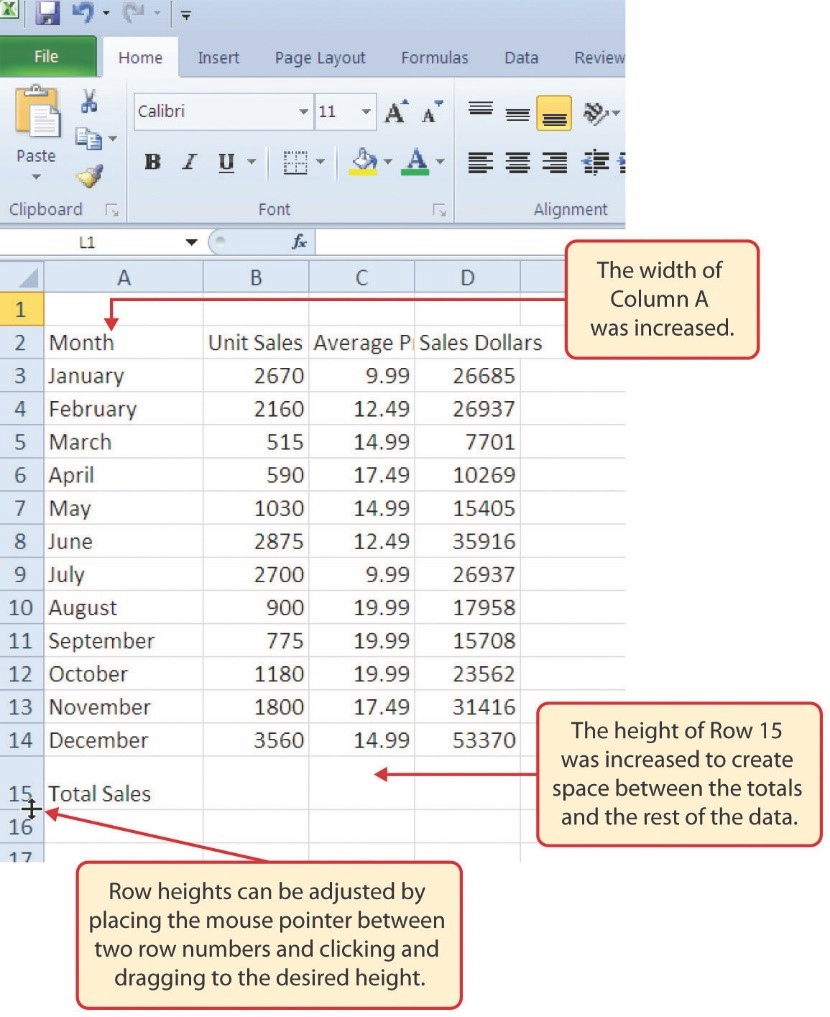
\includegraphics[width=\maxwidth{.95\linewidth}]{gfx/ch01_fig25}
	\caption{GMW Sales Data with Column A and Row 15 Adjusted}
	\label{01:fig25}
\end{figure}

\begin{center}
	\begin{sklbox}{Skill Refresher}
		\textbf{Adjusting Columns and Rows}
		\\
		\begin{itemize}
			\setlength{\itemsep}{0pt}
			\setlength{\parskip}{0pt}
			\setlength{\parsep}{0pt}
			
			\item Activate at least one cell in the row or column you are adjusting.
			\item Click the Home tab of the Ribbon.
			\item Click the Format button in the Cells group.
			\item Click either Row Height or Column Width from the drop-down menu.
			\item Enter the Row Height in points or Column Width in characters in the dialog box.
			\item Click the OK button.
			
		\end{itemize}
	\end{sklbox}
\end{center}

\subsection{Hiding Columns and Rows}

In addition to adjusting the columns and rows on a worksheet, you can also hide columns and rows. This is a useful technique for enhancing the visual appearance of a worksheet that contains data that is not necessary to display. These features will be demonstrated using the GMW Sales Data workbook. However, there is no need to have hidden columns or rows for this worksheet. The use of these skills here will be for demonstration purposes only.

\begin{enumerate}
	\item Click cell \textsf{C1} in the Sheet1 worksheet by placing the mouse pointer over the cell location and clicking the left mouse button.
	\item Click the Format button in the Home tab of the Ribbon.
	\item Place the mouse pointer over the Hide \& Unhide option in the drop-down menu. This will open a submenu of options.
	\item Click the Hide Columns option in the submenu of options (see Figure \ref{01:fig26}). This will hide Column \textsf{C}.
\end{enumerate}

\begin{figure}[H]
	\centering
	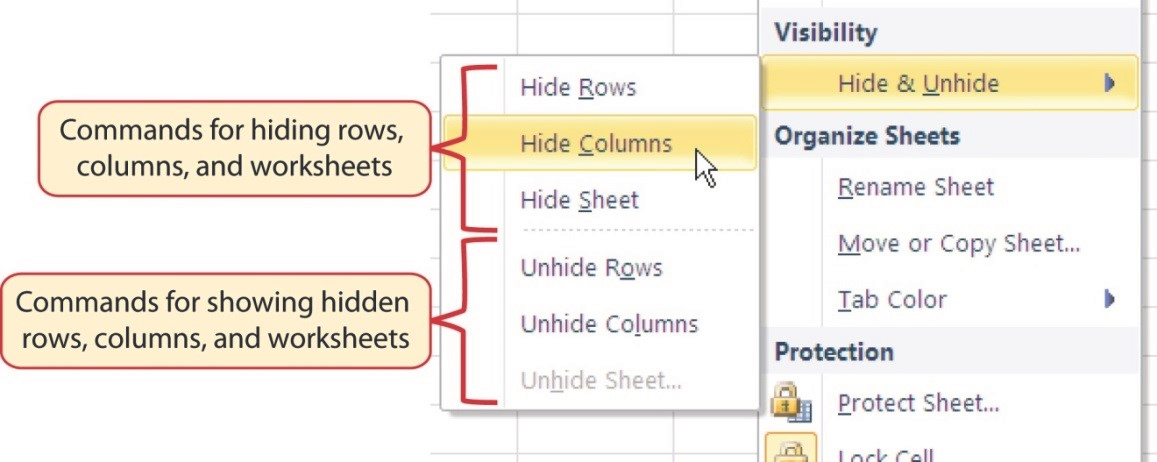
\includegraphics[width=\maxwidth{.95\linewidth}]{gfx/ch01_fig26}
	\caption{Hide \& Unhide Submenu}
	\label{01:fig26}
\end{figure}

\begin{center}
	\begin{shtcutbox}{Keyboard Shortcuts}
		\textbf{Hiding Columns}
		\\
		\begin{itemize}
			\setlength{\itemsep}{0pt}
			\setlength{\parskip}{0pt}
			\setlength{\parsep}{0pt}
			
			\item Hold down the \keystroke{Ctrl} key while pressing the number \keystroke{0} on your keyboard.
			
		\end{itemize}
	\end{shtcutbox}
\end{center}

Figure \ref{01:fig27} shows the workbook with Column \textsf{C} hidden in the Sheet1 worksheet. You can tell a column is hidden by the missing letter ``C.''

\begin{figure}[H]
	\centering
	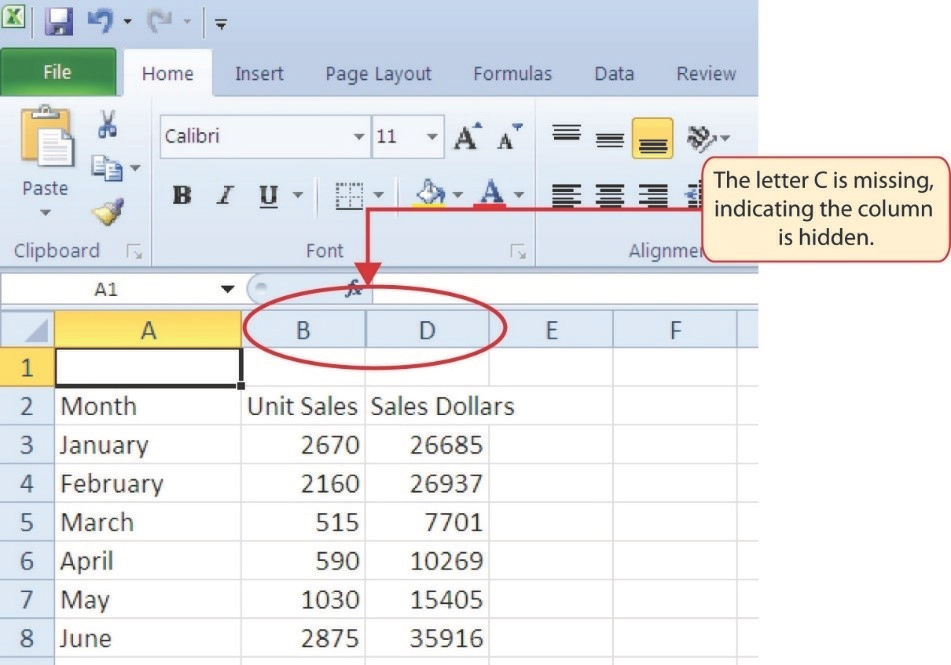
\includegraphics[width=\maxwidth{.95\linewidth}]{gfx/ch01_fig27}
	\caption{Hidden Column}
	\label{01:fig27}
\end{figure}

To unhide a column, use the following steps.

\begin{enumerate}
	\item Highlight the range \textsf{B1:D1} by activating cell \textsf{B1} and clicking and dragging over to cell \textsf{D1}.
	\item Click the Format button in the Home tab of the Ribbon.
	\item Place the mouse pointer over the Hide \& Unhide option in the drop-down menu.
	\item Click the Unhide Columns option in the submenu of options. Column \textsf{C} will now be visible on the worksheet.
\end{enumerate}

\begin{center}
	\begin{shtcutbox}{Keyboard Shortcuts}
		\textbf{Unhiding Columns}
		\\
		\begin{itemize}
			\setlength{\itemsep}{0pt}
			\setlength{\parskip}{0pt}
			\setlength{\parsep}{0pt}
			
			\item Highlight cells on either side of the hidden column(s), then hold down the \keystroke{Ctrl} key and the \keystroke{Shift} key while pressing the close parenthesis key, \keystroke{)}, on your keyboard.
			
		\end{itemize}
	\end{shtcutbox}
\end{center}

The following steps demonstrate how to hide rows, which is similar to hiding columns.

\begin{enumerate}
	\item Click cell \textsf{A3} in the Sheet1 worksheet by placing the mouse pointer over the cell location and clicking the left mouse button.
	\item Click the Format button in the Home tab of the Ribbon.
	\item Place the mouse pointer over the Hide \& Unhide option in the drop-down menu. This will open a submenu of options.
	\item Click the Hide Rows option in the submenu of options. This will hide Row 3.
\end{enumerate}

\begin{center}
	\begin{shtcutbox}{Keyboard Shortcuts}
		\textbf{Hiding Rows}
		\\
		\begin{itemize}
			\setlength{\itemsep}{0pt}
			\setlength{\parskip}{0pt}
			\setlength{\parsep}{0pt}
			
			\item Hold down the \keystroke{Ctrl} key while pressing the number \keystroke{9} key on your keyboard.
			
		\end{itemize}
	\end{shtcutbox}
\end{center}

To unhide a row, follow these steps.

\begin{enumerate}
	\item Highlight the range \textsf{A2:A4} by activating cell \textsf{A2} and clicking and dragging over to cell \textsf{A4}.
	\item Click the Format button in the Home tab of the Ribbon.
	\item Place the mouse pointer over the Hide \& Unhide option in the drop-down menu.
	\item Click the Unhide Rows option in the submenu of options. Row 3 will now be visible on the worksheet.
\end{enumerate}

\begin{center}
	\begin{shtcutbox}{Keyboard Shortcuts}
		\textbf{Unhiding Rows}
		\\
		\begin{itemize}
			\setlength{\itemsep}{0pt}
			\setlength{\parskip}{0pt}
			\setlength{\parsep}{0pt}
			
			\item Highlight cells above and below the hidden row(s), then hold down the \keystroke{Ctrl} key and the \keystroke{Shift} key while pressing the open parenthesis key, \keystroke{(}, on your keyboard.
			
		\end{itemize}
	\end{shtcutbox}
\end{center}

\begin{center}
	\begin{sklbox}{Skill Refresher}
		\textbf{Hiding Columns and Rows}
		\\
		\begin{itemize}
			\setlength{\itemsep}{0pt}
			\setlength{\parskip}{0pt}
			\setlength{\parsep}{0pt}
			
			\item Activate at least one cell in the row(s) or column(s) you are hiding.
			\item Click the Home tab of the Ribbon.
			\item Click the Format button in the Cells group.
			\item Place the mouse pointer over the Hide \& Unhide option.
			\item Click either the Hide Rows or Hide Columns option.
			
		\end{itemize}
	\end{sklbox}
\end{center}


\begin{center}
	\begin{sklbox}{Skill Refresher}
		\textbf{Unhiding Columns and Rows}
		\\
		\begin{itemize}
			\setlength{\itemsep}{0pt}
			\setlength{\parskip}{0pt}
			\setlength{\parsep}{0pt}
			
			\item Highlight the cells above and below the hidden row(s) or to the left and right of the hidden column(s).
			\item Click the Home tab of the Ribbon.
			\item Click the Format button in the Cells group.
			\item Place the mouse pointer over the Hide \& Unhide option.
			\item Click either the Unhide Rows or Unhide Columns option.
			
		\end{itemize}
	\end{sklbox}
\end{center}

\subsection{Inserting Columns and Rows}

Using Excel workbooks that have been created by others is a very efficient way to work because it eliminates the need to create data worksheets from scratch. However, you may find that to accomplish your goals, you need to add additional columns or rows of data. In this case, you can insert blank columns or rows into a worksheet. The following steps demonstrate how to do this.

\begin{enumerate}
	\item Click cell \textsf{C1} in the Sheet1 worksheet by placing the mouse pointer over the cell location and clicking the left mouse button.
	\item Click the down arrow on the Insert button in the Home tab of the Ribbon (see Figure \ref{01:fig28}).
\end{enumerate}

\begin{figure}[H]
	\centering
	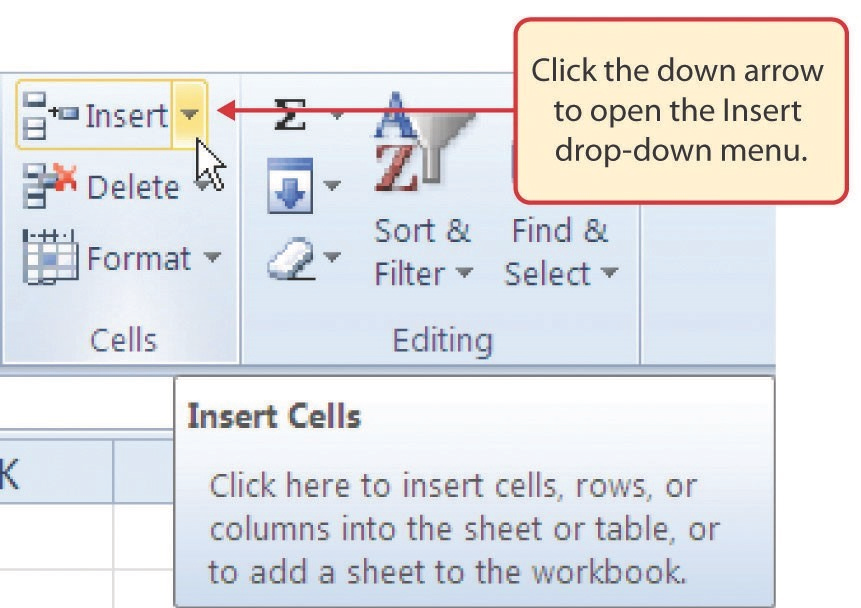
\includegraphics[width=\maxwidth{.95\linewidth}]{gfx/ch01_fig28}
	\caption{Insert Button (Down Arrow)}
	\label{01:fig28}
\end{figure}

\begin{center}
	\begin{infobox}{Integrity Check}
		\textbf{Hidden Rows and Columns}
		\\
		\\
		In most careers, it is common for professionals to use Excel workbooks that have been designed by a coworker. Before you use a workbook developed by someone else, always check for hidden rows and columns. You can quickly see whether a row or column is hidden if a row number or column letter is missing.
	\end{infobox}
\end{center}

\begin{enumerate}[resume]
	\item Click the Insert Sheet Columns option from the drop-down menu (see Figure \ref{01:fig29}). A blank column will be inserted to the left of Column \textsf{C}. The contents that were previously in Column \textsf{C} now appear in Column \textsf{D}. Note that columns are always inserted to the left of the activated cell.

\end{enumerate}

\begin{figure}[H]
	\centering
	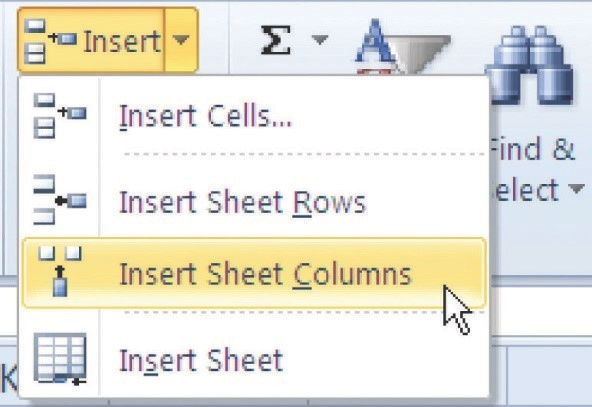
\includegraphics[width=\maxwidth{.95\linewidth}]{gfx/ch01_fig29}
	\caption{Insert Drop-Down Menu}
	\label{01:fig29}
\end{figure}

\begin{center}
	\begin{shtcutbox}{Keyboard Shortcuts}
		\textbf{Inserting Columns}
		\\
		\begin{itemize}
			\setlength{\itemsep}{0pt}
			\setlength{\parskip}{0pt}
			\setlength{\parsep}{0pt}
			
			\item Press the \keystroke{Alt} key and then the letters \keystroke{H}, \keystroke{I}, and \keystroke{C} one at a time. A column will be inserted to the left of the activated cell.One
			
		\end{itemize}
	\end{shtcutbox}
\end{center}

\begin{enumerate}[resume]
	\item Click cell \textsf{A3} in the Sheet1 worksheet by placing the mouse pointer over the cell location and clicking the left mouse button.
	\item Click the down arrow on the Insert button in the Home tab of the Ribbon (see Figure \ref{01:fig28}).
	\item Click the Insert Sheet Rows option from the drop-down menu (see Figure \ref{01:fig29}). A blank row will be inserted above Row 3. The contents that were previously in Row 3 now appear in Row 4. Note that rows are always inserted above the activated cell.
\end{enumerate}

\begin{center}
	\begin{shtcutbox}{Keyboard Shortcuts}
		\textbf{Inserting Rpws}
		\\
		\begin{itemize}
			\setlength{\itemsep}{0pt}
			\setlength{\parskip}{0pt}
			\setlength{\parsep}{0pt}
			
			\item Press the \keystroke{Alt} key and then the letters \keystroke{H}, \keystroke{I}, and \keystroke{R} one at a time. A row will be inserted above the activated cell.
			
		\end{itemize}
	\end{shtcutbox}
\end{center}

\begin{center}
	\begin{sklbox}{Skill Refresher}
		\textbf{Inserting Columns and Rows}
		\\
		\begin{itemize}
			\setlength{\itemsep}{0pt}
			\setlength{\parskip}{0pt}
			\setlength{\parsep}{0pt}
			
			\item Activate the cell to the right of the desired blank column or below the desired blank row.
			\item Click the Home tab of the Ribbon.
			\item Click the down arrow on the Insert button in the Cells group.
			\item Click either the Insert Sheet Columns or Insert Sheet Rows option.
			
		\end{itemize}
	\end{sklbox}
\end{center}


\subsection{Moving Data}

Once data are entered into a worksheet, you have the ability to move it to different locations. The following steps demonstrate how to move data to different locations on a worksheet.

\begin{enumerate}
	\item Highlight the range \textsf{D2:D15} by activating cell \textsf{D2} and clicking and dragging down to cell \textsf{D15}.
	\item Bring the mouse pointer to the left edge of cell \textsf{D2}. You will see the white block plus sign change to cross arrows (see Figure \ref{01:fig30}). This indicates that you can left click and drag the data to a new location.
\end{enumerate}

\begin{figure}[H]
	\centering
	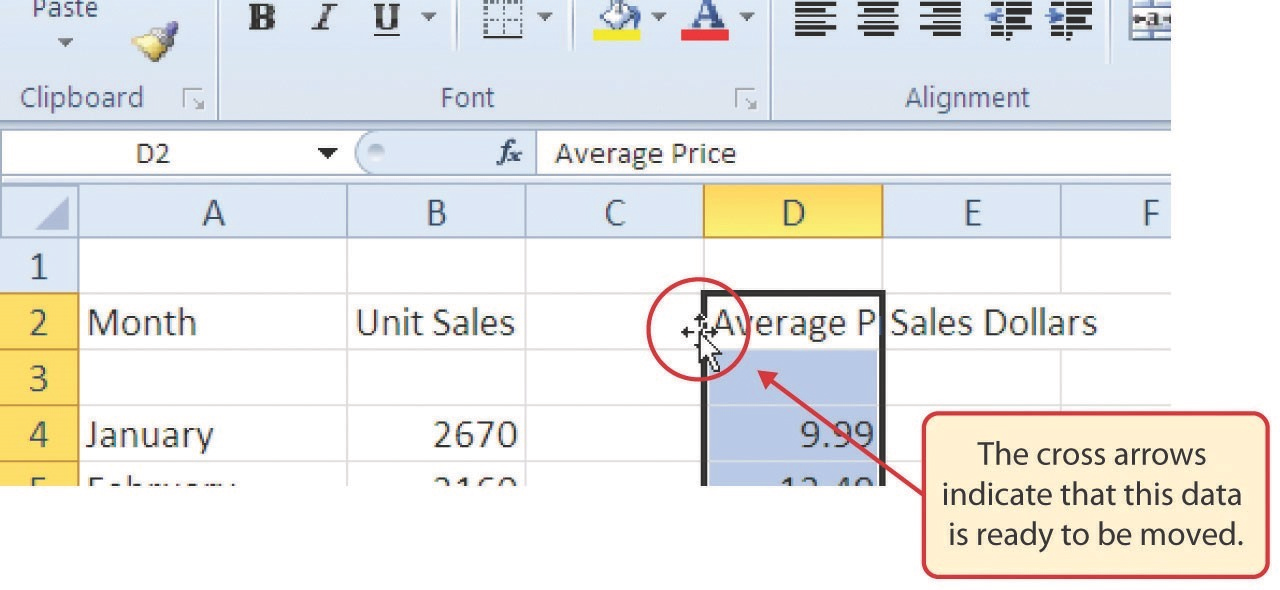
\includegraphics[width=\maxwidth{.95\linewidth}]{gfx/ch01_fig30}
	\caption{Moving Data}
	\label{01:fig30}
\end{figure}

\begin{enumerate}[resume]
	\item Left Click and drag the mouse pointer to cell \textsf{C2}.
	\item Release the left mouse button. The data now appears in Column \textsf{C}.
	\item Click the Undo button in the Quick Access Toolbar. This moves the data back to Column \textsf{D}.
\end{enumerate}

\begin{center}
	\begin{infobox}{Integrity Check}
		\textbf{Moving Data}
		\\
		\\
		Before moving data on a worksheet, make sure you identify all the components that belong with the series you are moving. For example, if you are moving a column of data, make sure the column heading is included. Also, make sure all values are highlighted in the column before moving it.
	\end{infobox}
\end{center}


\subsection{Deleting Columns and Rows}

You may need to delete entire columns or rows of data from a worksheet. This need may arise if you need to remove either blank columns or rows from a worksheet or columns and rows that contain data. The methods for removing cell contents were covered earlier and can be used to delete unwanted data. However, if you do not want a blank row or column in your workbook, you can delete it using the following steps.

\begin{enumerate}
	\item Click cell \textsf{A3} by placing the mouse pointer over the cell location and clicking the left mouse button.
	\item Click the down arrow on the Delete button in the Cells group in the Home tab of the Ribbon.
	\item Click the Delete Sheet Rows option from the drop-down menu (see Figure \ref{01:fig31}). This removes Row 3 and shifts all the data (below Row 2) in the worksheet up one row.
\end{enumerate}

\begin{figure}[H]
	\centering
	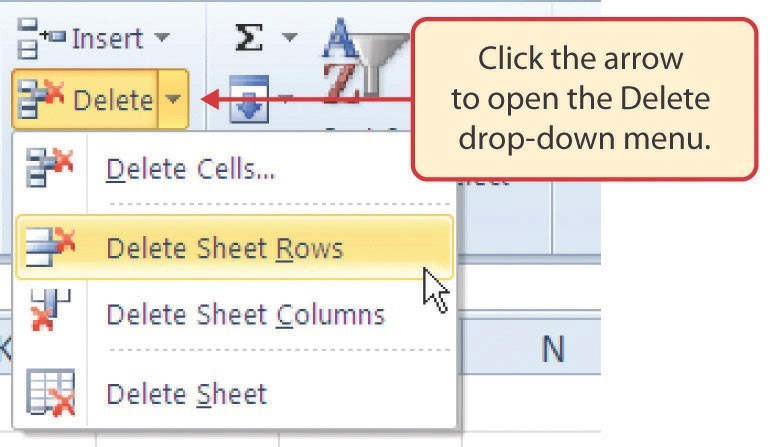
\includegraphics[width=\maxwidth{.95\linewidth}]{gfx/ch01_fig31}
	\caption{Delete Drop-Down Menu}
	\label{01:fig31}
\end{figure}

\begin{center}
	\begin{shtcutbox}{Keyboard Shortcuts}
		\textbf{Deleting Rows}
		\\
		\begin{itemize}
			\setlength{\itemsep}{0pt}
			\setlength{\parskip}{0pt}
			\setlength{\parsep}{0pt}
			
			\item Press the \keystroke{Alt} key and then the letters \keystroke{H}, \keystroke{D}, and \keystroke{R} one at a time. The row with the activated cell will be deleted.
			
		\end{itemize}
	\end{shtcutbox}
\end{center}

\begin{enumerate}[resume]
	\item Click cell C1 by placing the mouse pointer over the cell location and clicking the left mouse button.
	\item Click the down arrow on the Delete button in the Cells group in the Home tab of the Ribbon.
	\item Click the Delete Sheet Columns option from the drop-down menu (see Figure \ref{01:fig31}). This removes Column C and shifts all the data in the worksheet (to the right of Column B) over one column to the left.
	\item Save the changes to your workbook by clicking either the Save button on the Home ribbon; or by selecting the Save option from the File menu.
\end{enumerate}

\begin{center}
	\begin{shtcutbox}{Keyboard Shortcuts}
		\textbf{Deleting Columns}
		\\
		\begin{itemize}
			\setlength{\itemsep}{0pt}
			\setlength{\parskip}{0pt}
			\setlength{\parsep}{0pt}
			
			\item Press the \keystroke{Alt} key and then the letters \keystroke{H}, \keystroke{D}, and \keystroke{C} one at a time. The column with the activated cell will be deleted.
			
		\end{itemize}
	\end{shtcutbox}
\end{center}

\begin{center}
	\begin{sklbox}{Skill Refresher}
		\textbf{Deleting Columns and Rows}
		\\
		\begin{itemize}
			\setlength{\itemsep}{0pt}
			\setlength{\parskip}{0pt}
			\setlength{\parsep}{0pt}
			
			\item Activate any cell in the row or column that is to be deleted.
			\item Click the Home tab of the Ribbon.
			\item Click the down arrow on the Delete button in the Cells group.
			\item Click either the Delete Sheet Columns or the Delete Sheet Rows option.
			
		\end{itemize}
	\end{sklbox}
\end{center}

\begin{center}
	\begin{tkwbox}{Key Take-Aways}
		\textbf{Entering, Editing, and Managing Data}
		\\
		\begin{itemize}
			\setlength{\itemsep}{0pt}
			\setlength{\parskip}{0pt}
			\setlength{\parsep}{0pt}
			
			\item Column headings should be used in a worksheet and should accurately describe the data contained in each column.
			\item Using symbols such as dollar signs when entering numbers into a worksheet can slow down the data entry process.
			\item Worksheets must be carefully proofread when data has been manually entered.
			\item The Undo command is a valuable tool for recovering data that was deleted from a worksheet.
			\item When using a worksheet that was developed by someone else, look carefully for hidden columns or rows.
			
		\end{itemize}
	\end{tkwbox}
\end{center}

\section{Formatting and Data Analysis}

\begin{center}
	\begin{objbox}{Learning Objectives}
		\begin{itemize}
			\setlength{\itemsep}{0pt}
			\setlength{\parskip}{0pt}
			\setlength{\parsep}{0pt}
			
			\item Use formatting techniques as introduced in the Excel Spreadsheet Guidelines to enhance the appearance of a worksheet.
			\item Understand how to align data in cell locations.
			\item Examine how to enter multiple lines of text in a cell location.
			\item Understand how to add borders to a worksheet.
			\item Examine how to use the AutoSum feature to calculate totals.
			\item Use the Cut, Copy, and Paste commands to manipulate the data on a worksheet.
			\item 7. Understand how to move, rename, insert, and delete worksheet tabs.
		\end{itemize}
	\end{objbox}
\end{center}

This section addresses formatting commands that can be used to enhance the visual appearance of a worksheet. It also provides an introduction to mathematical calculations. The skills introduced in this section will give you powerful tools for analyzing the data that we have been working with in this workbook and will highlight how Excel is used to make key decisions in virtually any career. Additionally, Excel Spreadsheet Guidelines for format and appearance will be introduced as a format for the course and spreadsheets submitted.

\subsection{Formatting Data and Cells}

Enhancing the visual appearance of a worksheet is a critical step in creating a valuable tool for you or your coworkers when making key decisions. There are accepted professional formatting standards when spreadsheets contain only currency data. For this course, we will use the following Excel Guidelines for Formatting. The Figure \ref{01:fig32} displays how to use Accounting number format when ALL figures are currency. Only the first row of data and the totals should be formatted with the Accounting format. The other data should be formatted with Comma style. There also needs to be a Top Border above the numbers in the total row. If any of the numbers have cents, you need to format all of the data with two decimal places.

\begin{figure}[H]
	\centering
	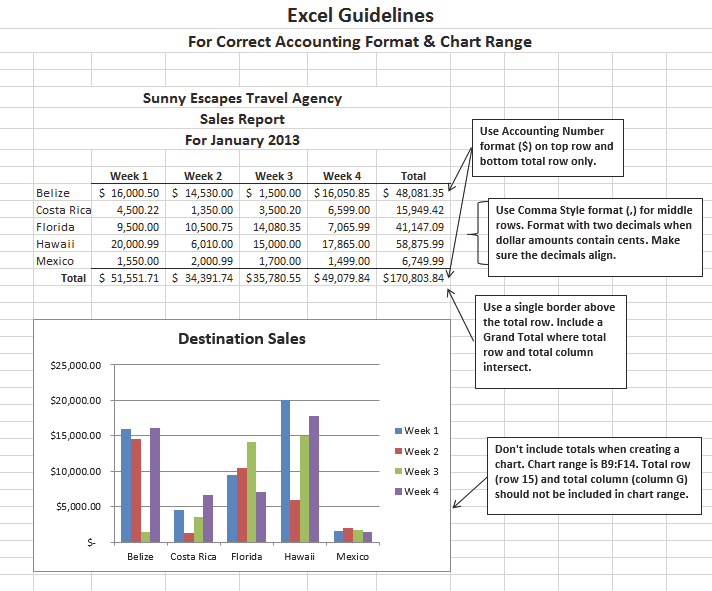
\includegraphics[width=\maxwidth{.95\linewidth}]{gfx/ch01_fig32}
	\caption{Excel Guidelines for Formatting Currency}
	\label{01:fig32}
\end{figure}

Often, your Excel spreadsheet will contain values that are both currency and non-currency in nature. When that is the case, use the guidelines in Figure \ref{01:fig33}.

\begin{figure}[H]
	\centering
	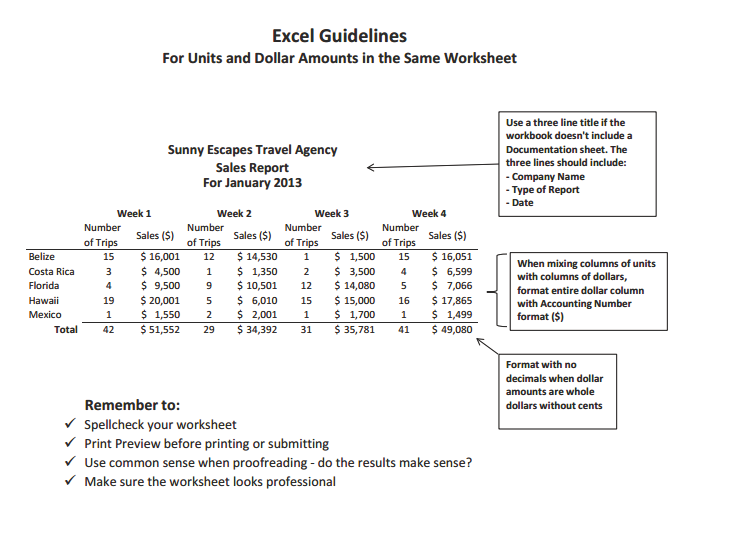
\includegraphics[width=\maxwidth{.95\linewidth}]{gfx/ch01_fig33}
	\caption{Excel Guidelines for Formatting Numbers}
	\label{01:fig33}
\end{figure}

The following steps demonstrate several fundamental formatting skills that will be applied to the workbook that we are developing for this chapter. Several of these formatting skills are identical to ones that you may have already used in other Microsoft applications such as Microsoft® Word® or
Microsoft® PowerPoint®.

\begin{enumerate}
	\item Highlight the range \textsf{A2:D2} in the \textbf{Sheet1} worksheet by placing the mouse pointer over cell \textsf{A2} and left clicking and dragging to cell \textsf{D2}. 
	\item Click the Bold button in the Font group of commands in the Home tab of the ribbon.
	\item Click the Border button in the Font group of commands in the Home tab of the Ribbon (see Figure \ref{01:fig34}). Select the Bottom Border option from the list to achieve the goal of a border on the bottom of row 2 below the column headings.
\end{enumerate}

\begin{figure}[H]
	\centering
	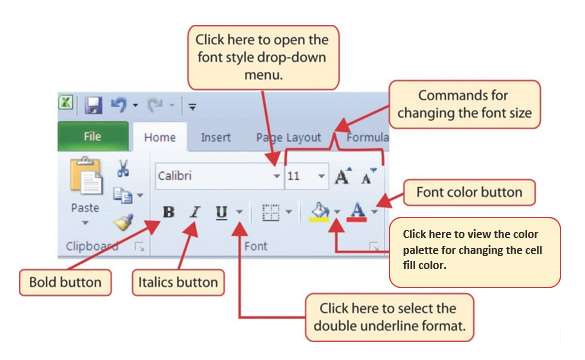
\includegraphics[width=\maxwidth{.95\linewidth}]{gfx/ch01_fig34}
	\caption{Font Group of Commands}
	\label{01:fig34}
\end{figure}

\begin{center}
	\begin{shtcutbox}{Keyboard Shortcuts}
		\textbf{Text Formats}
		\\
		\begin{itemize}
			\setlength{\itemsep}{0pt}
			\setlength{\parskip}{0pt}
			\setlength{\parsep}{0pt}
			
			\item Bold: hold the \keystroke{Ctrl} key while pressing the letter \keystroke{B} on your keyboard.
			\item Italics: hold the \keystroke{Ctrl} key while pressing the letter \keystroke{I} on your keyboard.
			\item Underline: hold the \keystroke{Ctrl} key while pressing the letter \keystroke{U} on your keyboard.
			
		\end{itemize}
	\end{shtcutbox}
\end{center}

\begin{enumerate}[resume]
	\item Highlight the range \textsf{A15:D15} by placing the mouse pointer over cell \textsf{A15} and left clicking and dragging to cell \textsf{D15}.
	\item Click the Bold button in the Font group of commands in the Home tab of the Ribbon.
	\item Click the Border button in the Font group of commands in the Home tab of the Ribbon. Select the Top Border option from the list to achieve the goal of a border on the top of row 15 where totals will eventually display.
	\item Highlight the range \textsf{B3:B14} by placing the mouse pointer over cell A and left clicking and dragging down to cell \textsf{B14}.
	\item Click the Comma Style button in the Number group of commands in the Home tab of the Ribbon. This feature adds a comma as well as two decimal places. (see Figure \ref{01:fig35}).
\end{enumerate}

\begin{figure}[H]
	\centering
	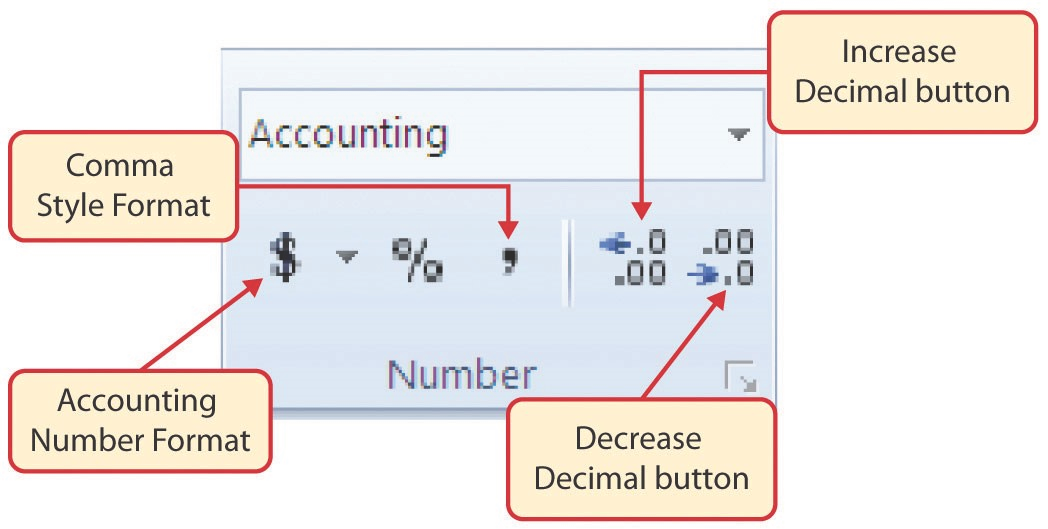
\includegraphics[width=\maxwidth{.95\linewidth}]{gfx/ch01_fig35}
	\caption{Number Group of Commands}
	\label{01:fig35}
\end{figure}

\begin{center}
	\begin{infobox}{Why?}
		\textbf{Format Column Headings and Totals}
		\\
		\\
		Applying formatting enhancements to the column headings and column totals in a worksheet is a very important technique, especially if you are sharing a workbook with other people. These formatting techniques allow users of the worksheet to clearly see the column headings that define the data. In addition, the column totals usually contain the most important data on a worksheet with respect to making decisions, and formatting techniques allow users to quickly see this information.
	\end{infobox}
\end{center}


\begin{enumerate}[resume]
	\item Since the figures in this range do not include cents, click the Decrease Decimal button in the Number group of commands in the Home tab of the Ribbon two times (see Figure \ref{01:fig35}).
	\item The numbers will also be reduced to zero decimal places.
	\item Highlight the range \textsf{C3:C14} by placing the mouse pointer over cell \textsf{C3} and left clicking and dragging down to cell \textsf{C14}.
	\item Click the Accounting Number Format button in the Number group of commands in the Home tab of the Ribbon (see Figure \ref{01:fig35}). This will add the US currency symbol and two decimal places to the values. This format is common when working with pricing data. As discussed above in the Formatting Data and Cells section, you will want to use Accounting format on all values in this range since the worksheet contains non-currency as well as currency data.
	\item Highlight the range \textsf{D3:D14} by placing the mouse pointer over cell \textsf{D3} and left clicking and dragging down to cell \textsf{D14}.
	\item Again, select the Accounting Number Format; this will add the US currency symbol to the values as well as two decimal places.
	\item Click the Decrease Decimal button in the Number group of commands in the Home tab of the Ribbon.
	\item This will add the US currency symbol to the values and reduce the decimal places to zero since there are no cents in these figures.
	\item Highlight the range \textsf{A1:D1} by placing the mouse pointer over cell \textsf{A1} and left clicking and dragging over to cell \textsf{D1}.
	\item Click the down arrow next to the Fill Color button in the Font group of commands in the Home tab of the Ribbon (see Figure \ref{01:fig36}). This will prepare the range for a worksheet title.
\end{enumerate}

\begin{figure}[H]
	\centering
	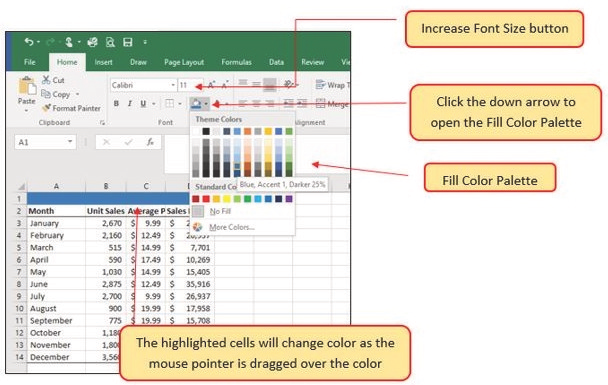
\includegraphics[width=\maxwidth{.95\linewidth}]{gfx/ch01_fig36}
	\caption{Fill Color Palette}
	\label{01:fig36}
\end{figure}

\begin{enumerate}[resume]
	\item Click the Blue, Accent 1, Darker 25\% color from the palette (see Figure \ref{01:fig36}). Notice that as you move the mouse pointer over the color palette, you will see a preview of how the color will appear in the highlighted cells. Experiment with this feature.
	\item Click on \textsf{A1} and enter the worksheet title: \textbf{General Merchandise World} and click on the check mark in the formula bar to enter this information.
	\item Since the black font is difficult to read on the blue background, change the font color to be more visible. Click the down arrow next to the Font Color button in the Font group of commands in the Home tab of the Ribbon and select White as the font color for this range (see Figure \ref{01:fig34}).
	\item Highlight the range \textsf{A1:D15} by placing the mouse pointer over cell \textsf{A1} and left clicking and dragging down to cell \textsf{D15}.
	\item Click the drop-down arrow on the right side of the Font button in the Home tab of the Ribbon; select Arial as the font for this range. (see Figure \ref{01:fig34}).
	\item Notice that as you move the mouse pointer over the font style options, you can see the font change in the highlighted cells.
	\item Expand the column width of Column \textsf{D} to 14 characters.
\end{enumerate}

Figure \ref{01:fig37} shows how the \textbf{Sheet1} worksheet should appear after the formatting techniques are applied.

\begin{figure}[H]
	\centering
	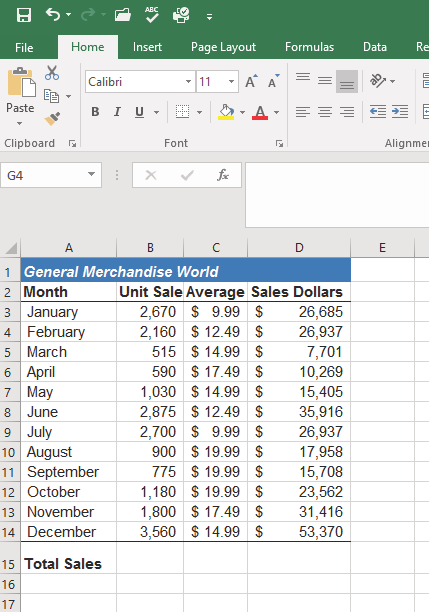
\includegraphics[width=\maxwidth{.95\linewidth}]{gfx/ch01_fig37}
	\caption{Formatting Techniques Applied}
	\label{01:fig37}
\end{figure}

\begin{center}
	\begin{infobox}{Why}
		\textbf{Pound Signs (\#\#\#\#) Appear in Columns}
		\\
		\\
		When a column is too narrow for a long number, Excel will automatically convert the number to a series of pound signs (\#\#\#\#). In the case of words or text data, Excel will only show the characters that fit in the column. However, this is not the case with numeric data because it can give the appearance of a number that is much smaller than what is actually in the cell. To remove the pound signs, increase the width of the column.
	\end{infobox}
\end{center}


\subsection{Data Alignment (Wrap Text, Merge Cells, and Center)}

The skills presented in this segment show how data are aligned within cell locations. For example, text and numbers can be centered in a cell location, left justified, right justified, and so on. In some cases you may want to stack multiword text entries vertically in a cell instead of expanding the width of a column. This is referred to as wrapping text. These skills are demonstrated in the following steps.

\begin{enumerate}
	\item 1. Highlight the range \textsf{B2:D2} by placing the mouse pointer over cell B2 and left clicking and dragging over to cell \textsf{D2}.
	\item Click the Center button in the Alignment group of commands in the Home tab of the Ribbon (see Figure \ref{01:fig38}). This will center the column headings in each cell location.
\end{enumerate}

\begin{figure}[H]
	\centering
	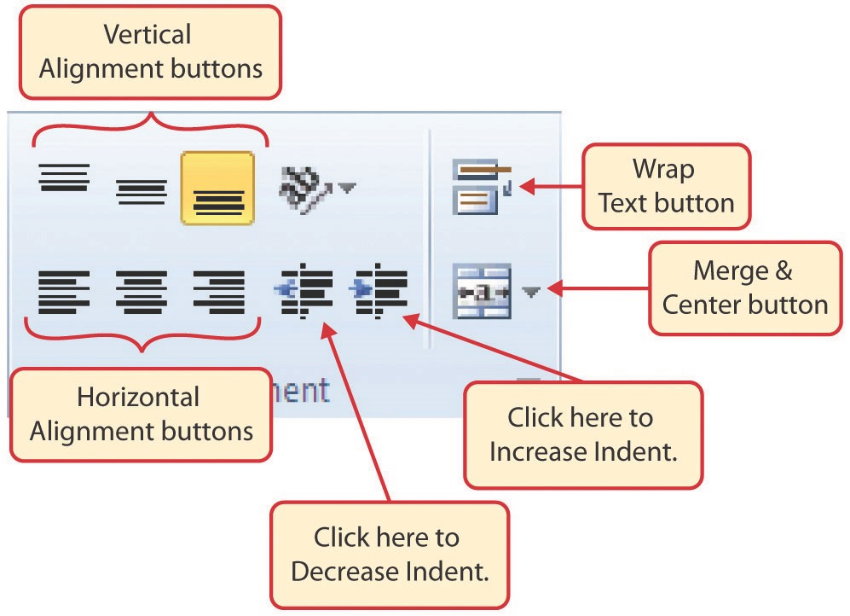
\includegraphics[width=\maxwidth{.95\linewidth}]{gfx/ch01_fig38}
	\caption{Alignment Group in Home Tab}
	\label{01:fig38}
\end{figure}

\begin{enumerate}[resume]
	\item Click the Wrap Text button in the Alignment group (see Figure \ref{01:fig38}). The height of Row 2 automatically expands, and the words that were cut off because the columns were too narrow are now stacked vertically.
\end{enumerate}

\begin{center}
	\begin{shtcutbox}{Keyboard Shortcuts}
		\textbf{Wrap Text}
		\\
		\begin{itemize}
			\setlength{\itemsep}{0pt}
			\setlength{\parskip}{0pt}
			\setlength{\parsep}{0pt}
			
			\item Press the \keystroke{Alt} key and then the letters \keystroke{H} and \keystroke{W} one at a time.
			
		\end{itemize}
	\end{shtcutbox}
\end{center}

\begin{enumerate}[resume]
	\item Highlight the range \textsf{A1:D1} by placing the mouse pointer over cell A1 and left clicking and dragging over to cell \textsf{D1}.
	\item Click the down arrow on the right side of the Merge \& Center button in the Alignment group of commands in the Home tab of the Ribbon.
	\item Left click the Merge \& Center option (see Figure \ref{01:fig39}). This will create one large cell location running across the top of the data set.

\end{enumerate}

\begin{figure}[H]
	\centering
	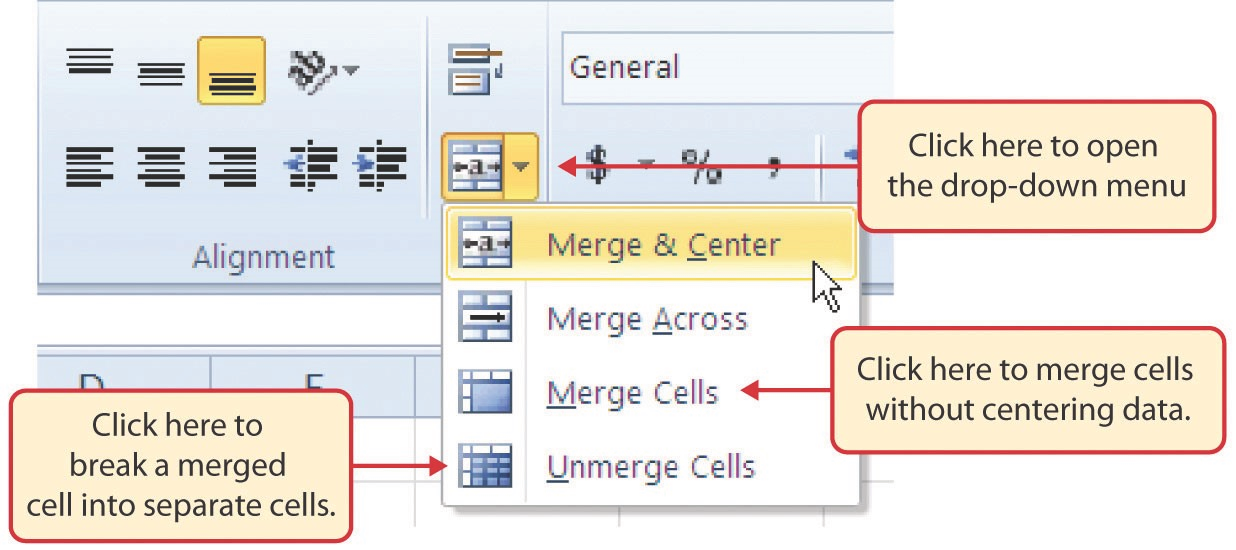
\includegraphics[width=\maxwidth{.95\linewidth}]{gfx/ch01_fig39}
	\caption{Merge Cell Drop-Down Menu}
	\label{01:fig39}
\end{figure}

\begin{center}
	\begin{shtcutbox}{Keyboard Shortcuts}
		\textbf{Merge Commands}
		\\
		\begin{itemize}
			\setlength{\itemsep}{0pt}
			\setlength{\parskip}{0pt}
			\setlength{\parsep}{0pt}
			
			\item Merge \& Center: Press the \keystroke{Alt} key and then the letters \keystroke{H}, \keystroke{M}, and \keystroke{C} one at a time.
			\item Merge Cells: Press the \keystroke{Alt} key and then the letters \keystroke{H}, \keystroke{M}, and \keystroke{M} one at a time.
			\item Unmerge Cells: Press the \keystroke{Alt} key and then the letters \keystroke{H}, \keystroke{M}, and \keystroke{U} one at a time.
			
		\end{itemize}
	\end{shtcutbox}
\end{center}

\begin{center}
	\begin{infobox}{Why?}
		\textbf{Wrap Text}
		\\
		\\
		The benefit of using the Wrap Text command is that it significantly reduces the need to expand the column width to accommodate multiword column headings. The problem with increasing the column width is that you may reduce the amount of data that can fit on a piece of paper or one screen. This makes it cumbersome to analyze the data in the worksheet and could increase the time it takes to make a decision.
	\end{infobox}
\end{center}

Figure \ref{01:fig40} shows the Sheet1 worksheet with the data alignment commands applied. The reason for merging the cells in the range \textsf{A1:D1} will become apparent in the next segment.

\begin{figure}[H]
	\centering
	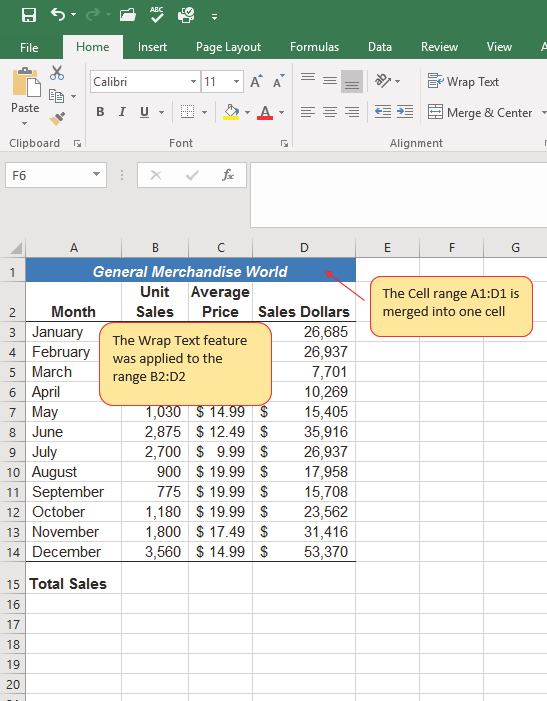
\includegraphics[width=\maxwidth{.95\linewidth}]{gfx/ch01_fig40}
	\caption{Sheet1 with Data Alignment Features Added}
	\label{01:fig40}
\end{figure}

\begin{center}
	\begin{infobox}{Why?}
		\textbf{Merge \& Center}
		\\
		\\
		One of the most common reasons the Merge \& Center command is used is to center the title of a worksheet directly above the columns of data. Once the cells above the column headings are merged, a title can be centered above the columns of data. It is very difficult to center the title over the columns of data if the cells are not merged.
	\end{infobox}
\end{center}

\begin{center}
	\begin{sklbox}{Skill Refresher}
		\textbf{Wrap Text}
		\\
		\begin{itemize}
			\setlength{\itemsep}{0pt}
			\setlength{\parskip}{0pt}
			\setlength{\parsep}{0pt}
			
			\item Activate the cell or range of cells that contain text data.
			\item Click the Home tab of the Ribbon.
			\item Click the Wrap Text button.

		\end{itemize}
	\end{sklbox}
\end{center}

\begin{center}
	\begin{sklbox}{Skill Refresher}
		\textbf{Merge Cells}
		\\
		\begin{itemize}
			\setlength{\itemsep}{0pt}
			\setlength{\parskip}{0pt}
			\setlength{\parsep}{0pt}
			
			\item Highlight a range of cells that will be merged.
			\item Click the Home tab of the Ribbon.
			\item Click the down arrow next to the Merge \& Center button.
			\item Select an option from the Merge \& Center list.
			
		\end{itemize}
	\end{sklbox}
\end{center}


\subsection{Entering Multiple Lines of Text}

In the Sheet1 worksheet, the cells in the range \textsf{A1:D1} were merged for the purposes of adding a title to the worksheet. This worksheet will contain both a title and a subtitle. The following steps explain how you can enter text into a cell and determine where you want the second line of text to begin.

\begin{enumerate}
	\item Activate cell \textsf{A1} in the Sheet1 worksheet by placing the mouse pointer over cell \textsf{A1} and clicking the left mouse button. Since the cells were merged, clicking cell \textsf{A1} will automatically activate the range \textsf{A1:D1}. Position your mouse to the end of the title, directly after the ``d'' in the word ``World'' and double-click to get a cursor (flashing I-beam).
	\item Hold down the \keystroke{Alt} key and press the \keystroke{Enter} key. This will start a new line of text in this cell location.
	\item 3. Type the text ``Retail Sales (in millions)'' and press the \keystroke{Enter} key.
	\item Select cell \textsf{A1}. Then click the Italics and Bold buttons in the Font group of commands in the Home tab of the Ribbon.
	\item Increase the height of Row 1 to 30 points. Once the row height is increased, all the text typed into the cell will be visible (see Figure \ref{01:fig41}).

\end{enumerate}

\begin{figure}[H]
	\centering
	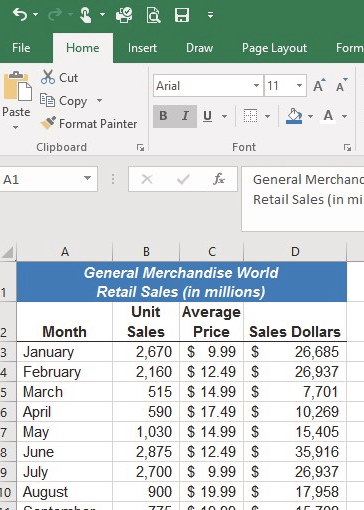
\includegraphics[width=\maxwidth{.95\linewidth}]{gfx/ch01_fig41}
	\caption{Title \& Subtitle Added to the Worksheet}
	\label{01:fig41}
\end{figure}

\begin{center}
	\begin{sklbox}{Skill Refresher}
		\textbf{Entering Multiple Lines of Text}
		\\
		\begin{itemize}
			\setlength{\itemsep}{0pt}
			\setlength{\parskip}{0pt}
			\setlength{\parsep}{0pt}
			
			\item Activate a cell location.
			\item Type the first line of text.
			\item Hold down the \keystroke{Alt} key and press the \keystroke{Enter} key.
			\item Type the second line of text and press the \keystroke{Enter} key.
			
		\end{itemize}
	\end{sklbox}
\end{center}

\subsection{Borders (Adding Lines to a Worksheet)}

In Excel, adding custom lines to a worksheet is known as adding borders. Borders are different from the grid lines that appear on a worksheet and that define the perimeter of the cell locations. The Borders command lets you add a variety of line styles to a worksheet that can make reading the worksheet much easier. The following steps illustrate methods for adding preset borders and custom borders to a worksheet.

\begin{enumerate}
	\item Click the down arrow to the right of the Borders button in the Font group of commands in the Home page of the Ribbon to view border options. (see Figure \ref{01:fig42}).
\end{enumerate}

\begin{figure}[H]
	\centering
	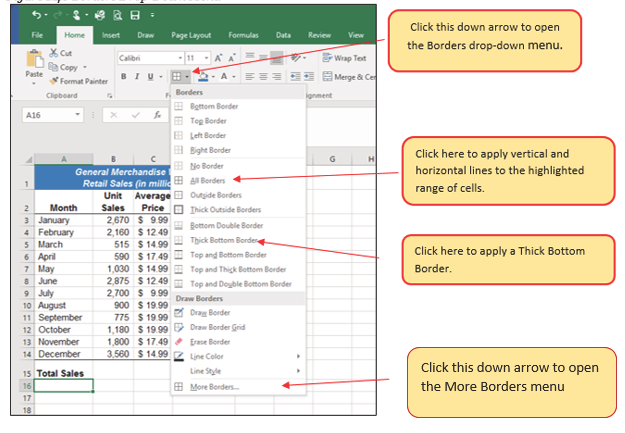
\includegraphics[width=\maxwidth{.95\linewidth}]{gfx/ch01_fig42}
	\caption{Borders Drop-Down Menu}
	\label{01:fig42}
\end{figure}

\begin{enumerate}[resume]
	\item 2. Highlight the range \textsf{A1:D15}. Left click the All Borders option from the Borders drop-down menu (see Figure \ref{01:fig42}). This will add vertical and horizontal lines to the range \textsf{A1:D15}.
	\item Highlight the range \textsf{A2:D2} by placing the mouse pointer over cell \textsf{A2} and left clicking and dragging over to cell \textsf{D2}.
	\item Click the down arrow to the right of the Borders button.
	\item Left click the Thick Bottom Border option from the Borders drop-down menu.
	\item Highlight the range \textsf{A14:D14} and apply a Thick Bottom Border from the drop-down menu. The thick border will help maintain the Excel Formatting Guidelines.
	\item Highlight the range \textsf{A1:D15}.
	\item Click the down arrow to the right of the Borders button.
	\item Click More Borders… at the bottom of the List.
	\item This will open the Format Cells dialog box (see Figure \ref{01:fig43}). You can access all formatting commands in Excel through this dialog box.
	\item In the Style section of the Borders tab, left click the thickest line style (see Figure \ref{01:fig43}).
	\item Left click the Outline button in the Presets section (see Figure \ref{01:fig43}).
	\item Click the OK button at the bottom of the dialog box (see Figure \ref{01:fig43}).
\end{enumerate}

\begin{figure}[H]
	\centering
	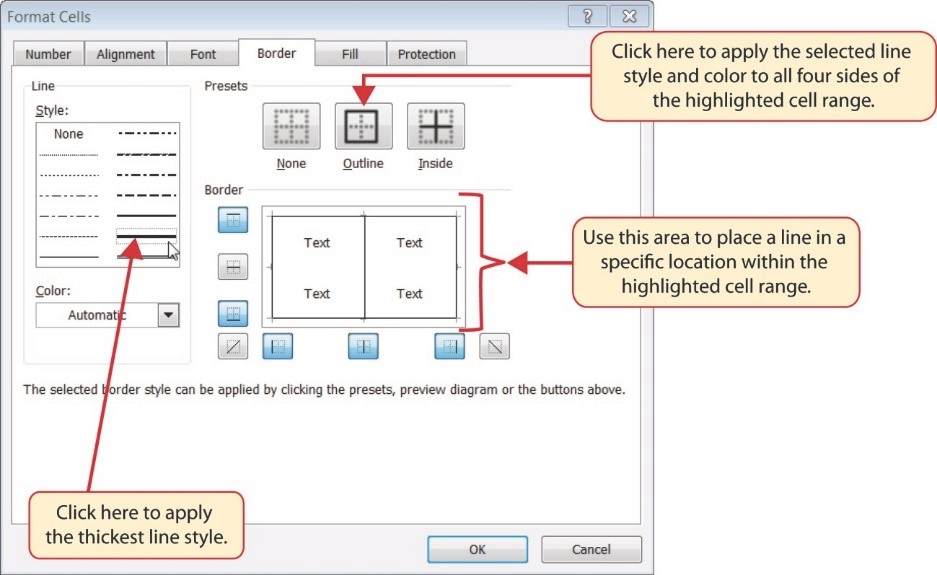
\includegraphics[width=\maxwidth{.95\linewidth}]{gfx/ch01_fig43}
	\caption{Borders Tab of the Format Cells Dialog Box}
	\label{01:fig43}
\end{figure}

The Sheet1 worksheet should now look like Figure \ref{01:fig44}.

\begin{figure}[H]
	\centering
	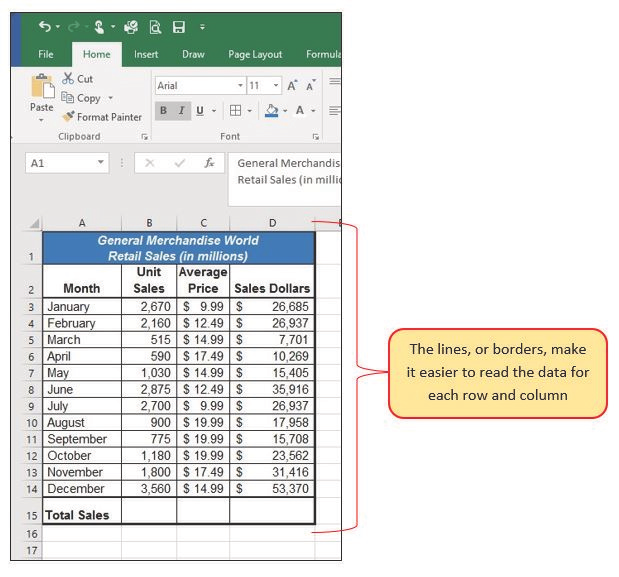
\includegraphics[width=\maxwidth{.95\linewidth}]{gfx/ch01_fig44}
	\caption{Borders Added to the Sheet1 Worksheet}
	\label{01:fig44}
\end{figure}

\begin{center}
	\begin{sklbox}{Skill Refresher}
		\textbf{Preset Borders}
		\\
		\begin{itemize}
			\setlength{\itemsep}{0pt}
			\setlength{\parskip}{0pt}
			\setlength{\parsep}{0pt}
			
			\item Highlight a range of cells that require borders.
			\item Click the Home tab of the Ribbon.
			\item Click the down arrow next to the Borders button.
			\item Select an option from the preset borders list.
			
		\end{itemize}

		\hfill \break
		\textbf{Custom Borders}
		\\
		\begin{itemize}
			\setlength{\itemsep}{0pt}
			\setlength{\parskip}{0pt}
			\setlength{\parsep}{0pt}
			
			\item Highlight a range of cells that require borders.
			\item Click the Home tab of the Ribbon.
			\item Click the down arrow next to the Borders button.
			\item Select the More Borders option at the bottom of the options list.
			\item Select a line style and line color.
			\item Select a placement option.
			\item Click the OK button on the dialog box.
			
		\end{itemize}

	\end{sklbox}
\end{center}

\subsection{Autosum}

You will see at the bottom of Figure \ref{01:fig44} that Row 15 is intended to show the totals for the data in this worksheet. Applying mathematical computations to a range of cells is accomplished through functions in Excel. Chapter 2, ``Mathematical Computations,'' will review mathematical formulas and functions in detail. However, the following steps will demonstrate how you can quickly sum the values in a column of data using the AutoSum command.

\begin{enumerate}
	\item Activate cell \textsf{B15} in the Sheet1 worksheet.
	\item Click the Formulas tab of the Ribbon.
	\item Click the down arrow below the AutoSum button in the Function Library group of commands (see Figure \ref{01:fig45}). Note that the AutoSum button can also be found in the Editing group of commands in the Home tab of the Ribbon.
\end{enumerate}

\begin{figure}[H]
	\centering
	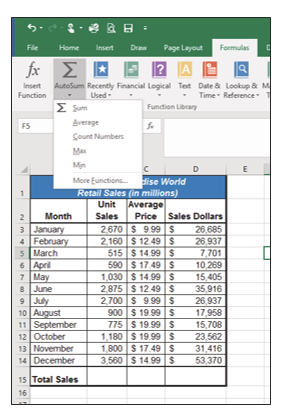
\includegraphics[width=\maxwidth{.95\linewidth}]{gfx/ch01_fig45}
	\caption{AutoSum Drop-Down List}
	\label{01:fig45}
\end{figure}

\begin{enumerate}[resume]
	\item Click the Sum option from the AutoSum drop-down menu. The first click will display a flashing marquee around the range. Click the check mark next to the Formula bar to complete the function.
	\item Excel will provide a total for the values in the Unit Sales column.
	\item Activate cell \textsf{D15}. It would not make sense to total the averages in column \textsf{C} so \textsf{C15} will be left blank.
	\item Repeat steps 3 through 5 to sum the values in the Sales Dollars column (see Figure \ref{01:fig46}).
\end{enumerate}

\begin{figure}[H]
	\centering
	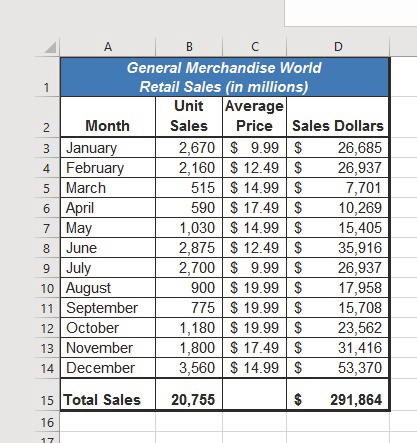
\includegraphics[width=\maxwidth{.95\linewidth}]{gfx/ch01_fig46}
	\caption{Totals Added to the Sheet1 Worksheet}
	\label{01:fig46}
\end{figure}

\begin{center}
	\begin{sklbox}{Skill Refresher}
		\textbf{AutoSum}
		\\
		\begin{itemize}
			\setlength{\itemsep}{0pt}
			\setlength{\parskip}{0pt}
			\setlength{\parsep}{0pt}
			
			\item Highlight a cell location below or to the right of a range of cells that contain numeric values.
			\item Click the Formulas tab of the Ribbon.
			\item Click the down arrow below the AutoSum button.
			\item Select a mathematical function from the list.
			
		\end{itemize}
	\end{sklbox}
\end{center}

\subsection{Moving, Renaming, Inserting, and Deleting Worksheets}

The default names for the worksheet tabs at the bottom of workbook are Sheet1, Sheet2, and so on. However, you can change the worksheet tab names to identify the data you are using in a workbook. Additionally, you can change the order in which the worksheet tabs appear in the workbook. The following steps explain how to rename and move the worksheets in a workbook.

\begin{enumerate}
	\item With the left mouse button, double click the Sheet1 worksheet tab at the bottom of the workbook (see Figure \ref{01:fig47}). Type the name \textbf{Sales by Month}.
	\item Press the \keystroke{Enter} key on your keyboard.
	\item With the left mouse button, double click the Sheet2 worksheet tab at the bottom of the workbook.
	\item Type the name \textbf{Unit Sales Rank} to prepare the worksheet for future use.
	\item Press the \keystroke{Enter} key on your keyboard.
\end{enumerate}

\begin{figure}[H]
	\centering
	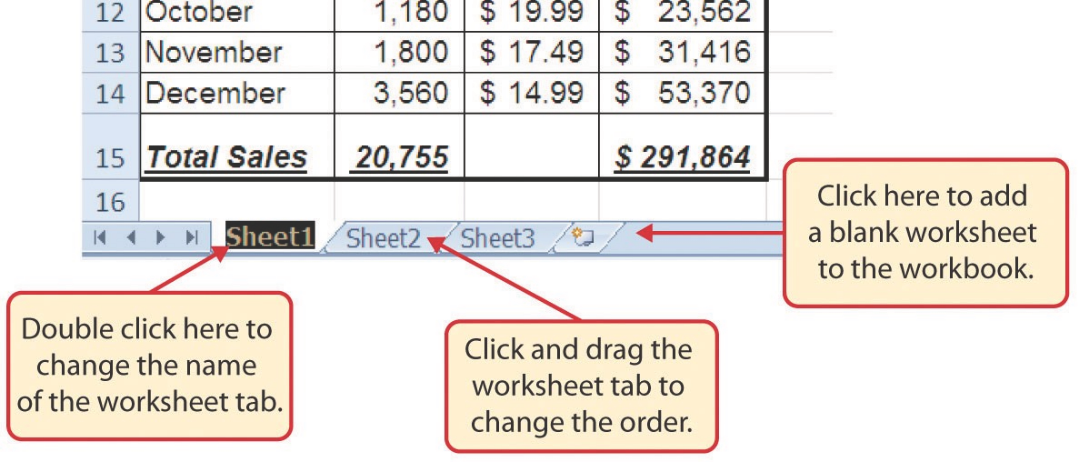
\includegraphics[width=\maxwidth{.95\linewidth}]{gfx/ch01_fig47}
	\caption{Renaming a Worksheet Tab}
	\label{01:fig47}
\end{figure}

\begin{enumerate}
	\item Click the Sheet3 worksheet tab.
	\item Click the Home tab of the Ribbon.
	\item Click the down arrow on the Delete button in the Cells group of commands.
	\item Click the Delete Sheet option from the drop-down list. This removes the unneeded worksheet.
	\item Click the Delete button on the Delete warning box (if a warning box appears).
	\item Complete the steps above to delete the newly named Unit Sales Rank worksheet since it is decided that worksheet is also unnecessary so that you are left with just one worksheet.
	\item Save the changes to your workbook by clicking either the Save button on the Home ribbon or by selecting the Save option from the File menu.
\end{enumerate}

\begin{center}
	\begin{infobox}{Integrity Check}
		\textbf{Deleting Worksheets}
		\\
		\\
		Be very cautious when deleting worksheets that contain data. Once a worksheet is deleted, you cannot use the Undo command to bring the sheet back. Deleting a worksheet is a permanent command.
	\end{infobox}
\end{center}

\begin{center}
	\begin{shtcutbox}{Keyboard Shortcuts}
		\textbf{Inserting New Worksheets}
		\\
		\begin{itemize}
			\setlength{\itemsep}{0pt}
			\setlength{\parskip}{0pt}
			\setlength{\parsep}{0pt}
			
			\item Press the \keystroke{Shift} key and then the \keystroke{F11} key on your keyboard.
			
		\end{itemize}
	\end{shtcutbox}
\end{center}


Figure \ref{01:fig48} shows the final appearance of the GMW Sales workbook.

\begin{figure}[H]
	\centering
	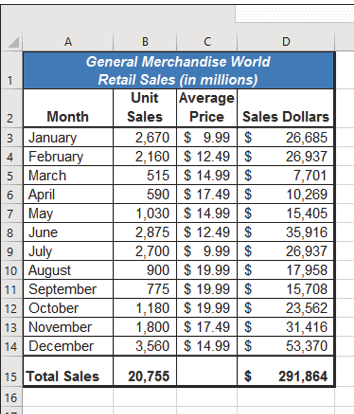
\includegraphics[width=\maxwidth{.95\linewidth}]{gfx/ch01_fig48}
	\caption{Final Appearance of the GMW Sales Workbook}
	\label{01:fig48}
\end{figure}

\begin{center}
	\begin{sklbox}{Skill Refresher}
		\textbf{Renaming Worksheets}
		\\
		\begin{itemize}
			\setlength{\itemsep}{0pt}
			\setlength{\parskip}{0pt}
			\setlength{\parsep}{0pt}
			
			\item Double click the worksheet tab.
			\item Type the new name.
			\item Press the \keystroke{Enter} key.
		\end{itemize}

		\hfill \break
		\textbf{Moving Worksheets}
		\\
		\begin{itemize}
			\setlength{\itemsep}{0pt}
			\setlength{\parskip}{0pt}
			\setlength{\parsep}{0pt}
			
			\item Left click the worksheet tab.
			\item Drag it to the desired position.
		\end{itemize}

		\hfill \break
		\textbf{Deleting Worksheets}
		\\
		\begin{itemize}
			\setlength{\itemsep}{0pt}
			\setlength{\parskip}{0pt}
			\setlength{\parsep}{0pt}
			
			\item Open the worksheet to be deleted.
			\item Click the Home tab of the Ribbon.
			\item Click the down arrow on the Delete button.
			\item Select the Delete Sheet option.
			\item Click Delete on the warning box.
		\end{itemize}

	\end{sklbox}
\end{center}

\begin{center}
	\begin{infobox}{Best Practice}
		\textbf{Summary Worksheet}
		\\
		\\
		It is considered a best practice to include a summary worksheet as the first sheet in the workbook. That sheet should include the purpose of the workbook and a brief explanation for each of the sheets in the book. It should also include contact information for the originator so questions that may come up later can be clarified.
	\end{infobox}
\end{center}


\begin{center}
	\begin{tkwbox}{Key Take-Aways}
		\textbf{Save}
		\\
		\begin{itemize}
			\setlength{\itemsep}{0pt}
			\setlength{\parskip}{0pt}
			\setlength{\parsep}{0pt}
			
			\item Formatting skills are critical for creating worksheets that are easy to read and have a professional appearance.
			\item A series of pound signs (\#\#\#\#) in a cell location indicates that the column is too narrow to display the number entered.
			\item Using the Wrap Text command allows you to stack multiword column headings vertically in a cell location, reducing the need to expand column widths.
			\item Use the Merge \& Center command to center the title of a worksheet directly over the columns that contain data.
			\item Adding borders or lines will make your worksheet easier to read and helps to separate the data in each column and row.
			\item You cannot use the Undo command to bring back a worksheet that has been deleted.
		
		\end{itemize}
	\end{tkwbox}
\end{center}

\section{Printing}

\begin{center}
	\begin{objbox}{Learning Objectives}
		\begin{itemize}
			\setlength{\itemsep}{0pt}
			\setlength{\parskip}{0pt}
			\setlength{\parsep}{0pt}
			
			\item Use the Page Layout tab to prepare a worksheet for printing.
			\item Add headers and footers to a printed worksheet.
			\item Examine how to print worksheets and workbooks.
		\end{itemize}
	\end{objbox}
\end{center}

Once you have completed a workbook, it is good practice to select the appropriate settings for printing. These settings are in the Page Layout tab of the Ribbon and discussed in this section of the chapter.

\subsection{Page Setup}

Before you can properly print the worksheets in a workbook, you must establish appropriate settings. The following steps explain several of the commands in the Page Layout tab of the Ribbon used to prepare a worksheet for printing.

\begin{enumerate}
	\item Open the \textbf{CH1 GMW Sales} workbook, if it is not already open.
	\item Click the Page Layout tab of the Ribbon.
	\item Click the Margins button in the Page Setup group of commands. This will open a drop-down list of options for setting the margins of your printed document.
	\item Click the Wide option from the Margins drop-down list. (see Figure \ref{01:fig49})
	\item Click the Orientation button in the Page Setup and select Landscape.
	\item Click on the arrow to the bottom right of the Page Setup category to launch the Page Setup options dialog box.
	\item Click the Margins tab and locate ``Center on Page''. Click the boxes to Horizontally and Vertically center the data on the worksheet. Click OK.

\end{enumerate}

\begin{figure}[H]
	\centering
	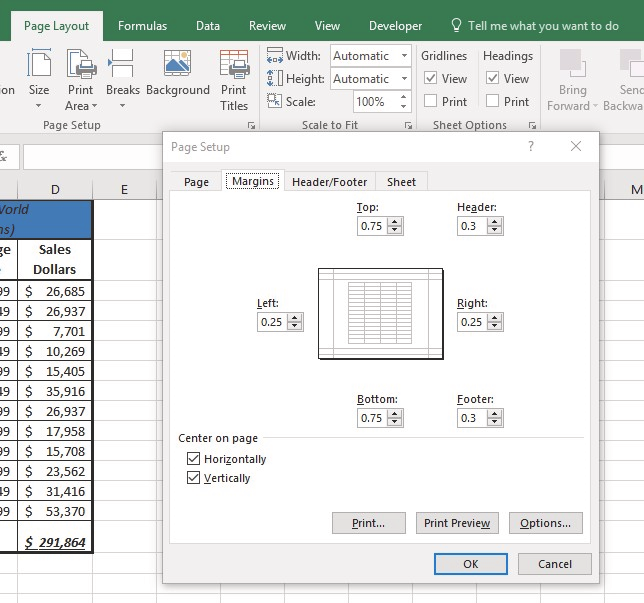
\includegraphics[width=\maxwidth{.95\linewidth}]{gfx/ch01_fig49}
	\caption{Page Layout Commands for Printing}
	\label{01:fig49}
\end{figure}

\begin{center}
	\begin{infobox}{Why?}
		\textbf{Use Print Settings}
		\\
		\\
		Because professionals often share Excel workbooks, it is a good practice to select the appropriate print settings in the Page Layout tab even if you do not intend to print the worksheets in a workbook. It can be extremely frustrating for recipients of a workbook who wish to print your worksheets to find that the necessary print settings have not been selected. This may reflect poorly on your attention to detail, especially if the recipient of the workbook is your boss.
	\end{infobox}
\end{center}

{\small
\begin{longtable}{p{0.75in}p{1.5in}p{1.5in}}
	\textbf{Command} & \textbf{Purpose} & \textbf{Use} \\
	\hline \endhead
	Margins & Sets the top, bottom, right, and left margin space for the printed document & 1. Click the Page Layout tab of the Ribbon.\newline2. Click the Margin button.\newline3. Click one of the preset margin options or click Custom Margins.\\
	\hline \\
	Orientation & Sets the orientation of the printed document to either portrait or landscape & 1. Click the Page Layout tab of the Ribbon.\newline2. Click the Orientation button.\newline3. Click one of the preset orientation options.\\
	\hline \\
	Size & Sets the paper size for the printed document & 1. Click the Page Layout tab of the Ribbon.\newline2. Click the Size button.\newline3. Click one of the preset paper size options or click More Paper Sizes. \\
	\hline \\
	Print Area & Used for printing only a specific area or range of cells on a worksheet & 1. Highlight the range of cells on a worksheet that you 		wish to print.\newline2. Click the Page Layout tab of the Ribbon.\newline3. Click the Print Area button.\newline4. Click the Set Print Area option from the drop-down list. \\
	\hline \\
	Breaks & Allows you to manually set the page breaks on a worksheet & 1. Activate a cell on the worksheet where the page break should be placed. Breaks are created above and to the left of the activated cell.\newline2. Click the Page Layout tab of the Ribbon.\newline3. Click the Breaks button.\newline4. Click the Insert Page Break option from the drop-down list. \\
	\hline \\
	Background & Adds a picture behind the cell locations in a worksheet & 1. Click the Page Layout tab of the Ribbon.\newline2. Click the Background button.\newline3. Select a picture stored on your computer or network. \\
	\hline \\
	Print Titles & Used when printing large data sets that are several pages long. This command will repeat the column headings at the top of each printed page. & 1. Click the Page Layout tab of the Ribbon.\newline2. Click the Print Titles button.\newline3. Click in the Rows to Repeat at Top input box in the Page Setup dialog box.\newline4. Click any cell in the row that contains the column headings for your worksheet.\newline5. Click the OK button at the bottom of the Page Setup dialog box. \\

	\caption{Purpose and Use for Page Setup Commands}
	\label{01:tab02}
\end{longtable}
}

\subsection{Headers and Footers}

When printing worksheets from Excel, it is common to add headers and footers to the printed document. Information in the header or footer could include the date, page number, file name, company name, and so on. The following steps explain how to add headers and footers to the GMW Sales Data workbook.

\begin{enumerate}
	\item Click the Insert Ribbon and click on Header \& Footer at the right end of the ribbon (located in the Text group). You will see the Design tab added to the Ribbon; this is used for creating the headers and footers for the printed worksheet. Also, this will convert the view of the worksheet from Normal to Page Layout (see Figure \ref{01:fig50}). This Page Layout view makes adding Headers \& Footers easy and provides key features to incorporate.
\end{enumerate}

\begin{figure}[H]
	\centering
	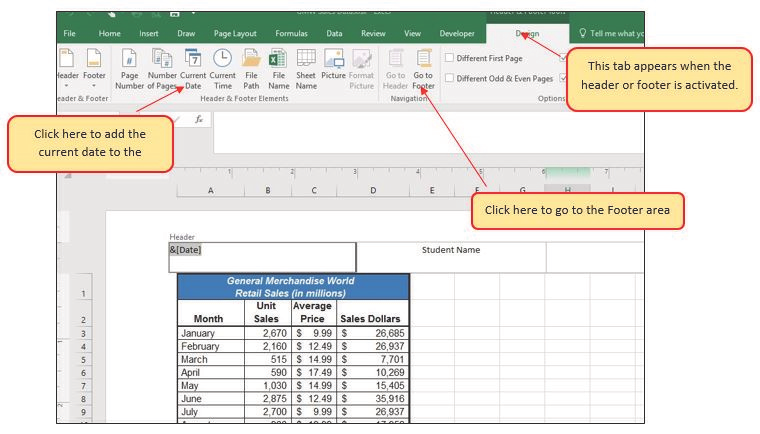
\includegraphics[width=\maxwidth{.95\linewidth}]{gfx/ch01_fig50}
	\caption{Design Tab for Creating Headers and Footers}
	\label{01:fig50}
\end{figure}

\begin{enumerate}[resume]
	\item Type your name in the center section of the Header.
	\item Place the mouse pointer over the left section of the Header and left click (see Figure \ref{01:fig50}).
	\item Click the Current Date button in the Header \& Footer Elements group of commands in the Design tab of the Ribbon. This view will display as \&[Date] until printed or until you return to normal view.
	\item Click the Go to Footer button in the Navigation group of commands in the Design tab of the Ribbon.
	\item Place the mouse pointer over the far right section of the footer and left click.
	\item Click the Page Number button (you may need to click on the Design tab again) in the Header \& Footer Elements group of commands in the Design tab of the Ribbon. This view will display as \&[Page] until printed or until you return to normal view.
	\item Click any cell location outside the header or footer area. The Design tab for creating headers and footers will disappear.
	\item Click the Normal view button in the lower right side of the Status Bar (see Figure \ref{01:fig51}).

\end{enumerate}

\begin{figure}[H]
	\centering
	\includegraphics[width=\maxwidth{.95\linewidth}]{gfx/ch01_fig51}
	\caption{Worksheet in Page Layout View}
	\label{01:fig51}
\end{figure}

\subsection{Printing Worksheets and Workbooks}

Once you have established the print settings for the worksheets in a workbook and have added headers and footers, you are ready to print your worksheets. The following steps explain how to print the worksheets in the GMW Sales workbook.

\begin{enumerate}
	\item Click the File tab on the Ribbon.
	\item Click the Print option on the left side of the Backstage view (see Figure \ref{01:fig52}). On the right side of the Backstage view, you will be able to see a preview of your printed worksheet.
\end{enumerate}

\begin{figure}[H]
	\centering
	\includegraphics[width=\maxwidth{.95\linewidth}]{gfx/ch01_fig52}
	\caption{Backstage View Print option}
	\label{01:fig52}
\end{figure}

\begin{enumerate}[resume]
	\item Click the Print Active Sheets button in the Print section of the Backstage view (see Figure \ref{01:fig52}).
	\item If your instructor has asked you to print your work, click the Print button.
	\item Click the Home tab of the Ribbon.
	\item Save and close the \textbf{CH1 GMW Sales} workbook.
	\item Compare your work with the self-check answer key (found in the Course Files link) and then submit the \textbf{CH1 GMW Sales} workbook as directed by your instructor.
\end{enumerate}

\begin{center}
	\begin{tkwbox}{Key Take-Aways}
		\textbf{Print}
		\\
		\begin{itemize}
			\setlength{\itemsep}{0pt}
			\setlength{\parskip}{0pt}
			\setlength{\parsep}{0pt}

			\item The commands in the Page Layout tab of the Ribbon are used to prepare a worksheet for printing.
			\item You can add headers and footers to a worksheet to show key information such as page numbers, the date, the file name, your name, and so on.
			\item The Print commands are in the File tab of the Ribbon.
			
		\end{itemize}
	\end{tkwbox}
\end{center}

\section{Chapter Practice}

To assess your understanding of the material covered in the chapter, complete the following assignment.

\subsection{Basic Monthly Budget for Medical Office}

\textit{Download Data File: PR1 Data}

Creating and maintaining budgets are common practices in many careers. Budgets play a critical role in helping a business or household control expenditures. In this exercise you will create a budget for a hypothetical medical office while reviewing the skills covered in this chapter.

\begin{enumerate}
	\item Open the file name \textbf{PR1 Data}, then Save As \textbf{PR1 Medical Office Budget}.
	\item Activate all the cell locations in the Sheet1 worksheet by left clicking the Select All button in the upper left corner of the worksheet (See Figure \ref{01:fig53}).
\end{enumerate}

\begin{figure}[H]
	\centering
	\includegraphics[width=\maxwidth{.95\linewidth}]{gfx/ch01_fig53}
	\caption{The Select All Button}
	\label{01:fig53}
\end{figure}


\begin{enumerate}[resume]
	\item In the Home tab of the Ribbon, set the font style to Arial and the font size to 12 points. Then click any cell to deselect.
	\item Increase the width of Column \textsf{A} so all the entries in the range \textsf{A3:A8} are visible. Place the mouse pointer between the letter \textit{A} and letter \textit{B} of Column \textsf{A} and Column \textsf{B}. When the mouse pointer changes to a double arrow, left click and drag it to the right until the character width is approximately 18.00.
	\item Enter \textbf{Quarter 1} in cell \textsf{B2}.
	\item Use AutoFill to complete the headings in the range \textsf{C2:E2}. Activate cell \textsf{B2} and place the mouse pointer over the Fill Handle. When the mouse pointer changes to a black plus sign, left click and drag it to cell \textsf{E2}.
	\item Highlight the range \textsf{B2:E2} and click the Format button in the Home tab of the Ribbon. Click the Column Width option, type 11.57 in the Column Width dialog box, and then click the OK button in the Column Width dialog box.
	\item Enter the words \textbf{Medical Office Budget} in cell \textsf{A1}.
	\item Insert a blank column between Columns \textsf{A} and \textsf{B} by clicking on any cell in Column A. Then, click the drop-down arrow of the Insert button in the Home tab of the Ribbon. Click the Insert Sheet Columns option.
	\item Enter the words \textbf{Budget Cost} in cell \textsf{B2}.
	\item Adjust the width of Column \textsf{B} to approximately 13.29 characters.
	\item Highlight the range \textsf{A1:F1} and click the Merge \& Center button in the Home tab of the Ribbon to merge the cells in that range.
	\item Make the following format adjustments to the range \textsf{A1:F1}: bold; italics; change the font size to 14 points; change the cell fill color to Aqua, Accent 5, Darker 50\%; and change the font color to white.
	\item Increase the height of Row 1 to approximately 24.75 points.
	\item Make the following format adjustment to the range \textsf{A2:F2}: bold; and change the cell fill color to Tan, Background 2, Darker 10\%. Center the column titles so that they are horizontally centered in each cell.
	\item Set the alignment in cell \textsf{B2} to Wrap Text. Select \textsf{B2} and choose the Wrap Text button in the Home tab of the Ribbon.
	\item Copy cell \textsf{C3} and paste the contents into the range \textsf{D3:F3}.
	\item Copy the contents in the range \textsf{C6:C8} by highlighting the range and clicking the Copy button in the Home tab of the Ribbon. Then, highlight the range \textsf{D6:F8} and click the Paste button in the Home tab of the Ribbon.
	\item Calculate the total budget for all four quarters for the salaries. Activate cell \textsf{B3} and click the down arrow on the AutoSum button in the Formulas tab of the Ribbon. Click the Sum option from the drop-down list. Then, highlight the range \textsf{C3:F3} and press the \keystroke{Enter} key on the keyboard.
	\item Copy the formula in cell \textsf{B3} and paste them into the range \textsf{B4:B8}.
	\item Format the range \textsf{B3:F8} with Accounting format and zero decimal places.
	\item Highlight the range \textsf{A1:F8} and click the down arrow next to the Borders button in the Home tab of the Ribbon. Select the All Borders option from the drop-down list.
	\item Double click the Sheet1 worksheet tab to change the name of Sheet1 to the word \textbf{Budget}, and press the \keystroke{Enter} key. Delete any unnecessary worksheets.
	\item Change the orientation of the Budget worksheet so it prints landscape instead of portrait.
	\item Use Fit to 1 page so the Budget worksheet prints on one piece of paper, if it does not already.
	\item Add a header to the Budget worksheet that shows the date in the upper left corner and your name in the center.
	\item Add a footer to the Budget worksheet that shows the page number in the lower right corner. 
	\item Save \textbf{PR1 Medical Office Budget} workbook.
	\item Compare your work with the self-check answer key and then submit the \textbf{PR1 Medical Office Budget} workbook as directed by your instructor.
\end{enumerate}

\section{Scored Assessment}

\subsection{Sales and Inventory Items}

\textit{Download Data File: SC1 Data}

A key activity for marketing professionals is to analyze projected sales and inventory information. This is especially important for retail environments. This exercise utilizes the skills covered in this chapter to analyze sales and inventory data.

\begin{enumerate}
	\item Open the file named \textbf{SC1 Data} and then Save As \textbf{SC1 Sales and Inventory}
	\item In the Sheet1 worksheet, enter the word \textbf{Totals} in cell \textsf{C14}.
	\item Format all the cells in Sheet1 to Century font style and a 12-point font size.
	\item Set the column width for Columns \textsf{A} through \textsf{G} to 13.5.
	\item Edit the entry in cell \textsf{B2} to read ``Item Number.''
	\item Use AutoFill to fill the Item Numbers from \textsf{B3} into the range \textsf{B4:B13}. The item numbers should increase by one as they are filled through the range.
	\item Copy the contents of cell \textsf{A3} and paste them into the range \textsf{A4:A8}.
	\item Delete Column \textsf{F}.
	\item Format the range \textsf{A1:F2} so the text is Bold.
	\item Set the alignment in the range \textsf{A2:F2} to Wrap Text.
	\item Prepare \textsf{A1:F1} for the title text by changing the fill color of the cells in the range \textsf{A1:F1} to Red, Accent 2, Darker 25\%.
	\item Make the following font changes to the range \textsf{A1:F1}: set the font color to white, add italics, and set the font size to 14.
	\item Merge and center the cells in the range \textsf{A1:F1}.
	\item Enter the title for this worksheet in the range \textsf{A1:F1}. The title should appear on two lines. The first line should read \textbf{Status Report}. The second line should read \textbf{Sales and Inventory by Item}.
	\item Increase the height of Row 1 so the entire title is visible.
	\item Format the values in the range \textsf{C3:C13} with dollar signs and two decimal places.
	\item Format the values in the range \textsf{E3:F13} with comma style, zero decimal places.
	\item In cell \textsf{E14}, use AutoSum to calculate the sum of the values in the range \textsf{E3:E13}.
	\item In cell \textsf{F14}, use AutoSum to calculate the sum of the values in the range \textsf{F3:F13}.
	\item Apply All Borders to the range \textsf{A1:F14}.
	\item Add a thick bottom border to row 2; add a thick bottom border to row 13.
	\item Add a thick line border around the perimeter of the range \textsf{A1:F14}.
	\item Insert a new blank worksheet in the workbook (this will be Sheet4).
	\item Delete Sheet3.
	\item Move Sheet4 ahead of Sheet2 so the order of the worksheets is Sheet1, Sheet4, and Sheet2.
	\item Rename the Sheet1 worksheet tab to ``Status Report.''
	\item Change the orientation of the Status Report worksheet so it prints landscape instead of portrait.
	\item Add a header to the Status Report worksheet that shows the date (needs to update) in the upper left corner and your name in the center.
	\item Add a footer to the Status Report worksheet that shows the page number in the lower right corner with the word ``Page'' before the number.
	\item Center the worksheet both horizontally and vertically on the sheet.
	\item Save the \textbf{SC1 Sales and Inventory} workbook.
	\item Submit the \textbf{SC1 Sales and Inventory} workbook as directed by your instructor.

\end{enumerate}
